\documentclass[9pt]{beamer}

\mode<presentation>
{
  \usetheme{EastLansing}

  \setbeamercovered{transparent}
}


\usepackage[english]{babel}
\usepackage{times}
\usepackage[T1]{fontenc}
\usepackage{fontspec}
\usepackage{booktabs}
\usepackage{tikz}
\usepackage{pgfplots}
\usepackage{float}
\usepackage{algorithm}
\usepackage{algorithmic}
\usepackage{textpos}
\usepackage{cancel}
\usepackage{csquotes}
\usepackage[backend=biber,style=authoryear-comp,autocite=inline,maxcitenames=99,maxbibnames=99,uniquename=false,mincrossrefs=99,dashed=false]{biblatex}

\usetikzlibrary{arrows,positioning,automata,bayesnet}

\pgfplotsset{compat=1.16}
\addbibresource{journals.bib}
\addbibresource{proceedings.bib}
\addbibresource{references.bib}

\setmainfont{Gill Sans}[ItalicFont={Gill Sans Italic}]

\setbeamertemplate{navigation symbols}{}

\graphicspath{{graphics/}}

\title[Bayesian neural networks for sparse coding]
{Bayesian neural networks for sparse coding}

\author[Danil Kuzin]{{Danil~Kuzin \inst{1} \and Olga Isupova \inst{2} \and Lyudmila Mihaylova \inst{1}}}

\institute[]
{
  \inst{1} Department of Automatic Control and Systems Engineering, University of Sheffield, UK \and %
  \inst{2} Machine Learning Research Group, University of Oxford, UK \\
}

\date[2019]
{ICASSP 2019}


\pgfdeclareimage[height=1cm]{sheffield-logo}{graphics/logo}
%\logo{\pgfuseimage{sheffield-logo}\vspace{220pt}}

\addtobeamertemplate{frametitle}{}{%
\begin{textblock*}{50mm}(.85\textwidth,-1cm)
\pgfuseimage{sheffield-logo}
\end{textblock*}}

% Delete this, if you do not want the table of contents to pop up at
% the beginning of each subsection:
% \AtBeginSubsection[]
%  {
%    \begin{frame}<beamer>{Outline}
%      \tableofcontents[currentsection,currentsubsection]
%    \end{frame}
%  }


% \AtBeginSubsection[]
% {
%   \begin{frame}<beamer>
%     \frametitle{Outline}
%     \tableofcontents[currentsubsection]
%   \end{frame}
% }


\begin{document}

\begin{frame}
  \titlepage
\end{frame}

%\begin{frame}{Outline}
%  \tableofcontents
%  % You might wish to add the option [pausesections]
%\end{frame}


\graphicspath{{graphics/intro/}}
\def \tikzdir {graphics/intro/}
\section{Introduction}

\subsection[Motivation]{Motivation}
\begin{frame}{Problem}
  \begin{columns}
    \begin{column}{0.5\textwidth}
      \begin{block}{Sparse regression}
        \begin{align*}
          &\mathbf{y} = \mathbf{X}\boldsymbol\beta + \boldsymbol\varepsilon, \\
          &\mathbf{y}\in\mathbb{R}^K, \,\boldsymbol\beta\in\mathbb{R}^D, \, K< D
        \end{align*}
        How to find sparse $\boldsymbol\beta$ given $\mathbf{y}$, $\mathbf{X}$?
      \end{block}
%      \begin{block}{Sparse methods}
%        \begin{itemize}
%          \item variable selection
%          \item sparse coding
%          \item sparse approximations
%        \end{itemize}
%      \end{block}
%
%      \begin{block}{Challenges}
%        \begin{itemize}
%          \item computationally intensive
%          \item structural assumptions
%          \item uncertainty estimation
%        \end{itemize}
%      \end{block}
    \end{column}

    \begin{column}{0.5\textwidth}
      \centering
      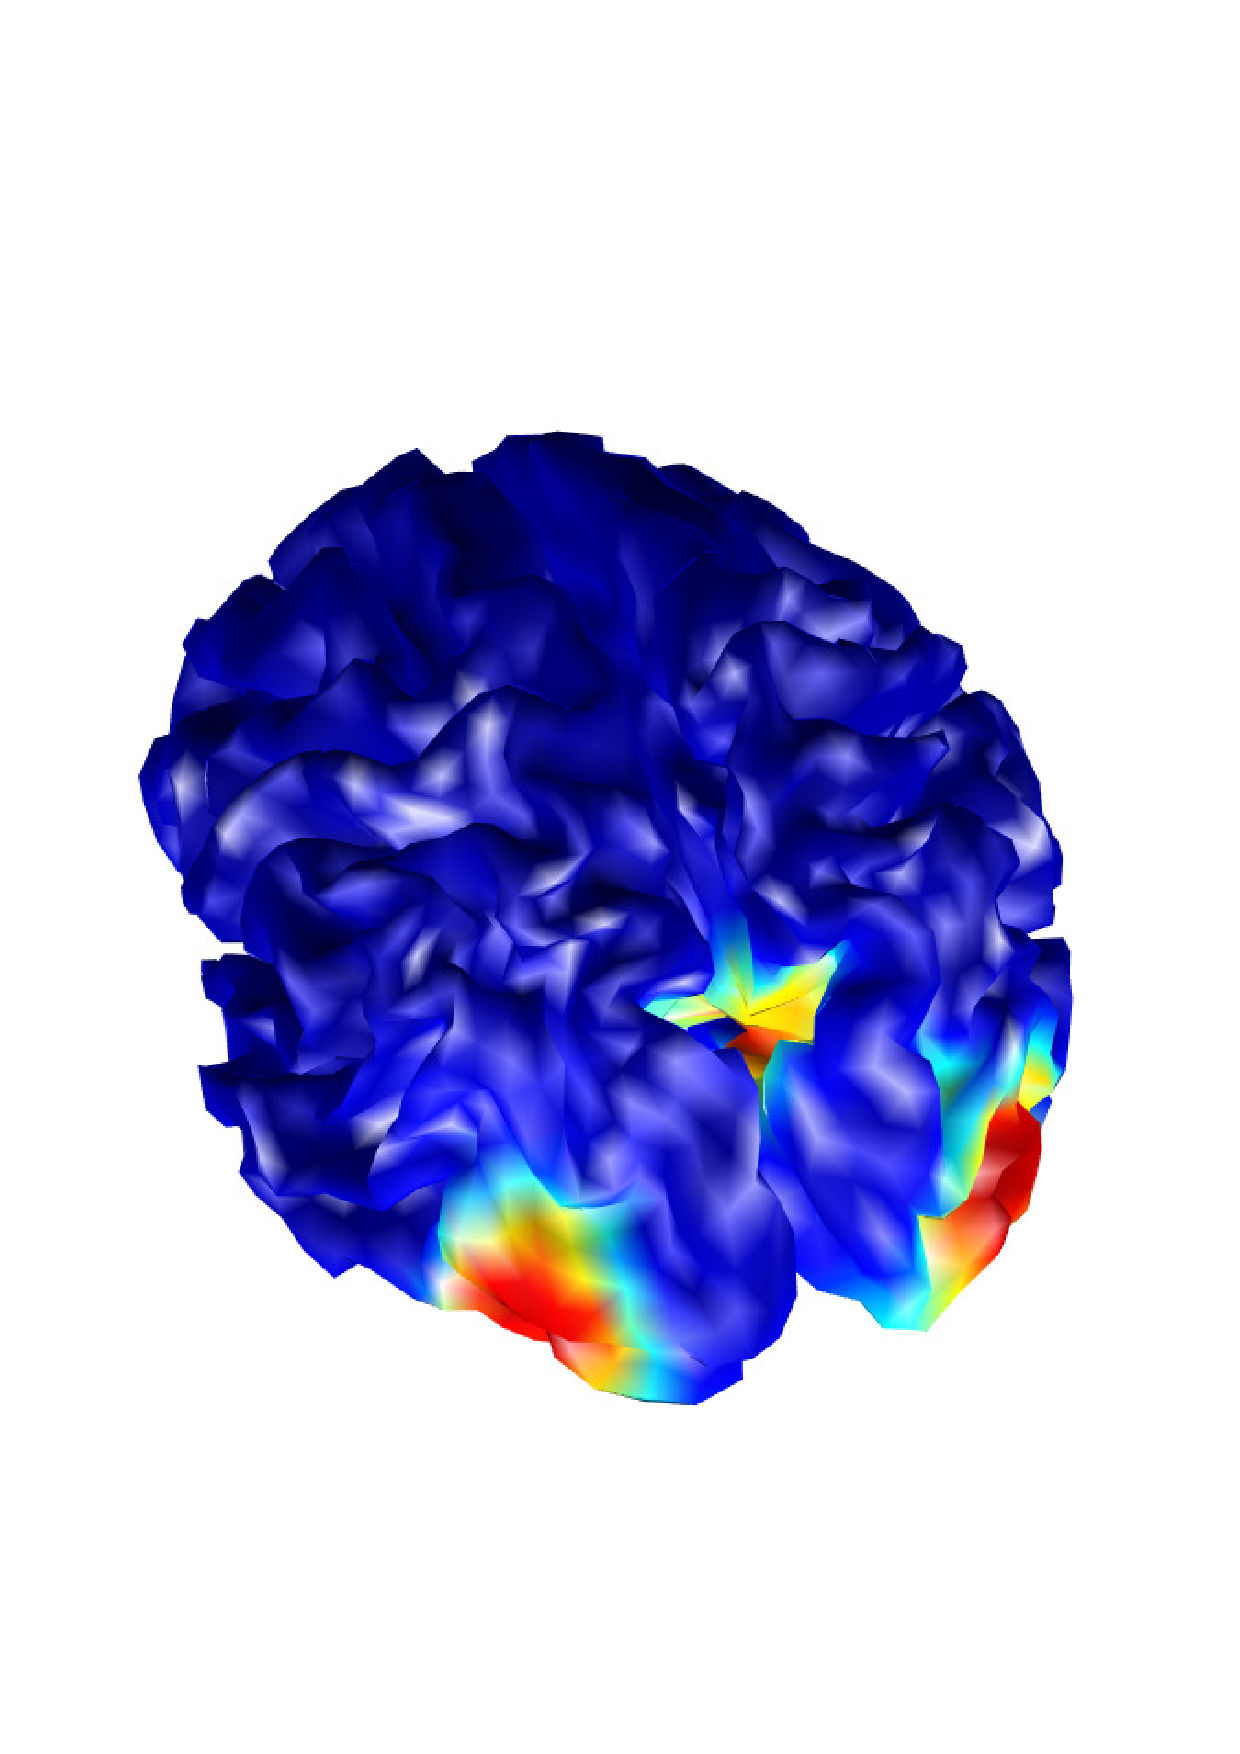
\includegraphics[width=0.33\textwidth]{andersen-eeg}
      \hfil
      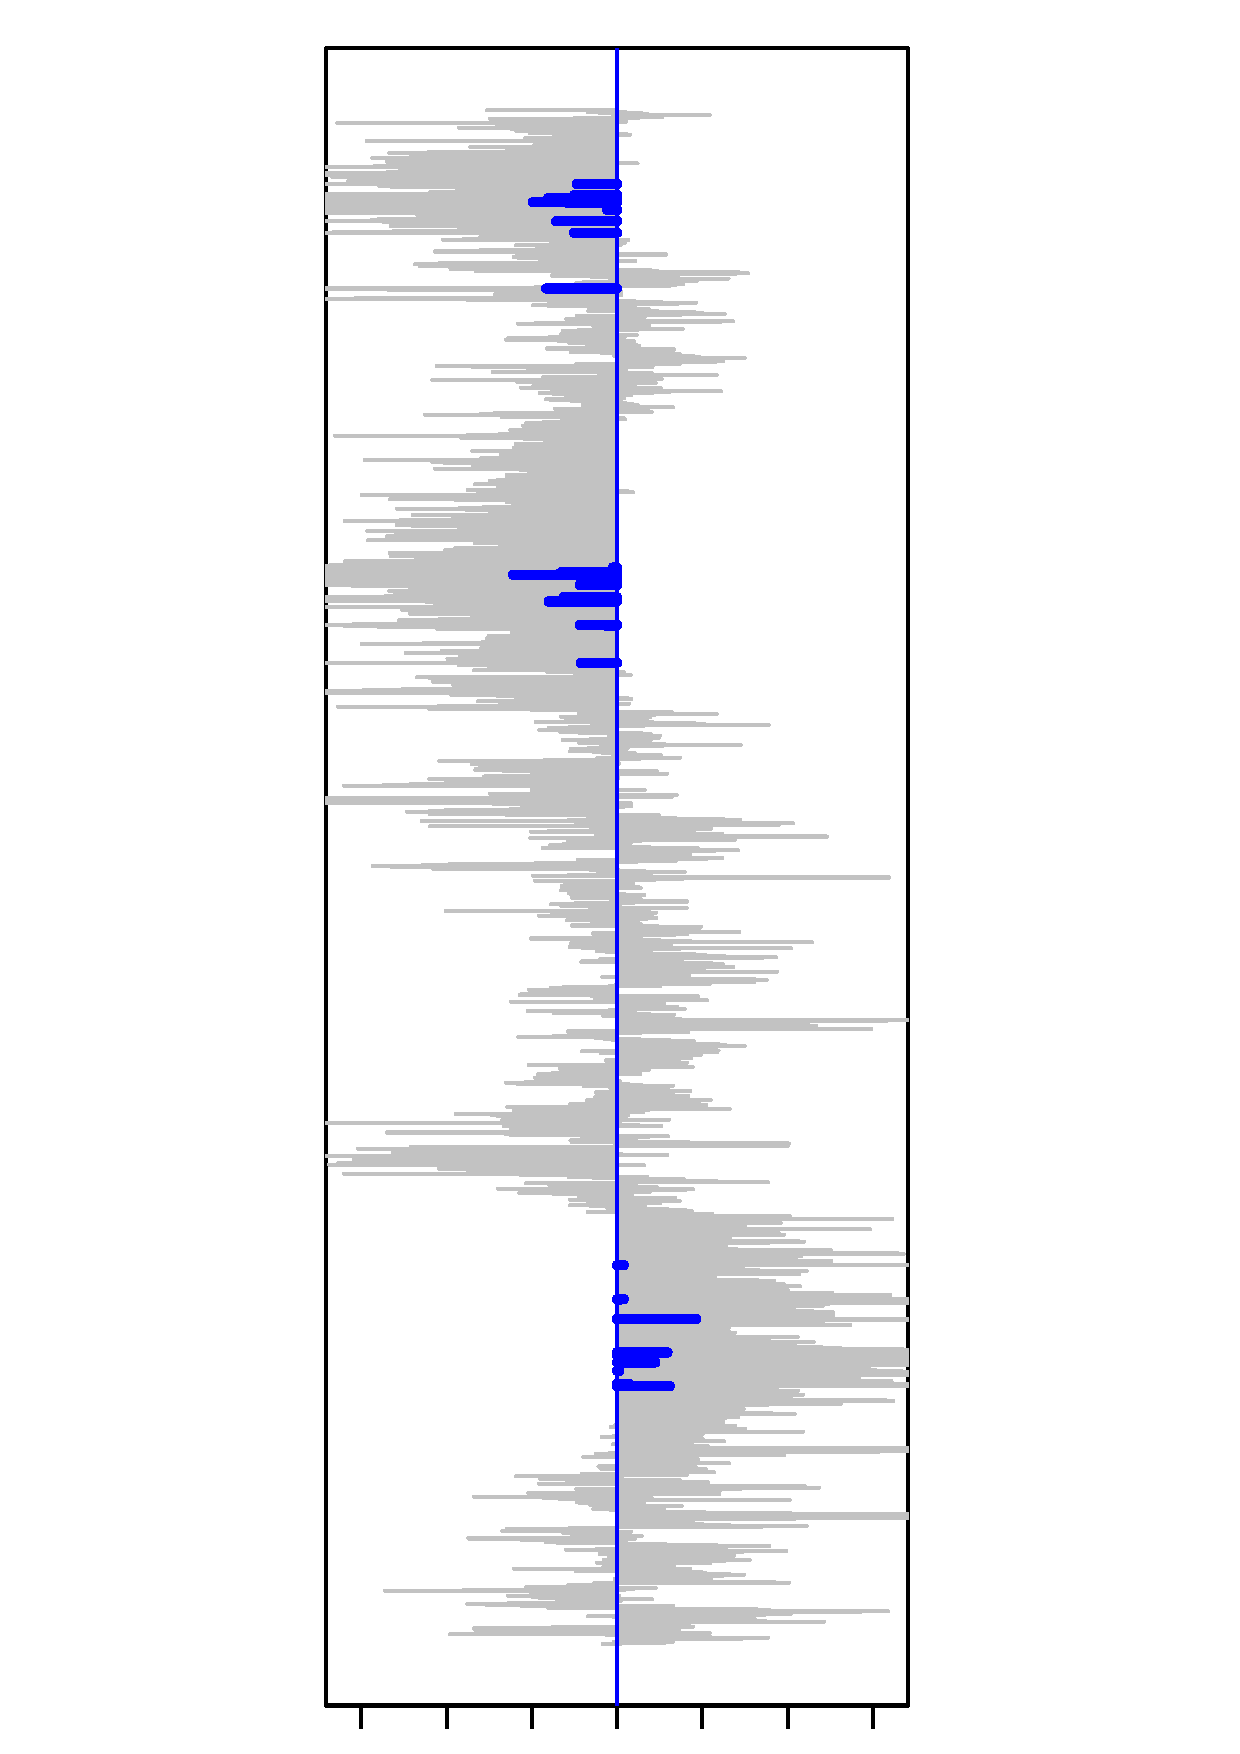
\includegraphics[width=0.33\textwidth]{sls-genome}
      \hfil
      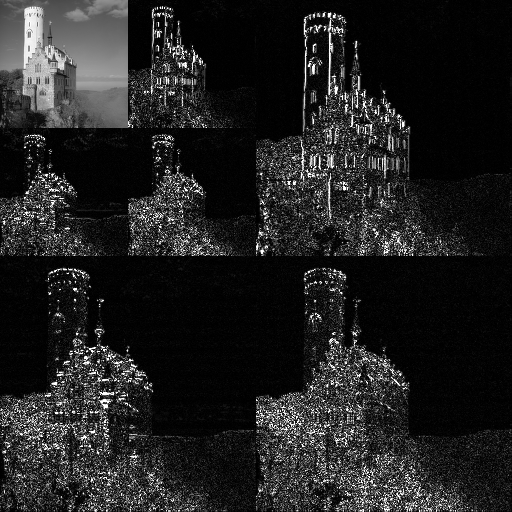
\includegraphics[width=0.45\textwidth]{wavelet_transform}
    \end{column}
  \end{columns}
\end{frame}

\subsection[Existing Solutions]{Existing Solutions}
\begin{frame}{Sparse frequentist regression}
  Add \alert{sparsity-inducing penalty}
  \begin{equation*}
    \widehat{\boldsymbol\beta} = \underset{\boldsymbol\beta}{\operatorname{argmin}}\left[||\mathbf{y} - \mathbf{X}\boldsymbol\beta||_2^2 + ||\boldsymbol\beta||_p^p\right]
  \end{equation*}
  \centering
  \begin{columns}
    \begin{column}{0.25\textwidth}
      \centering
      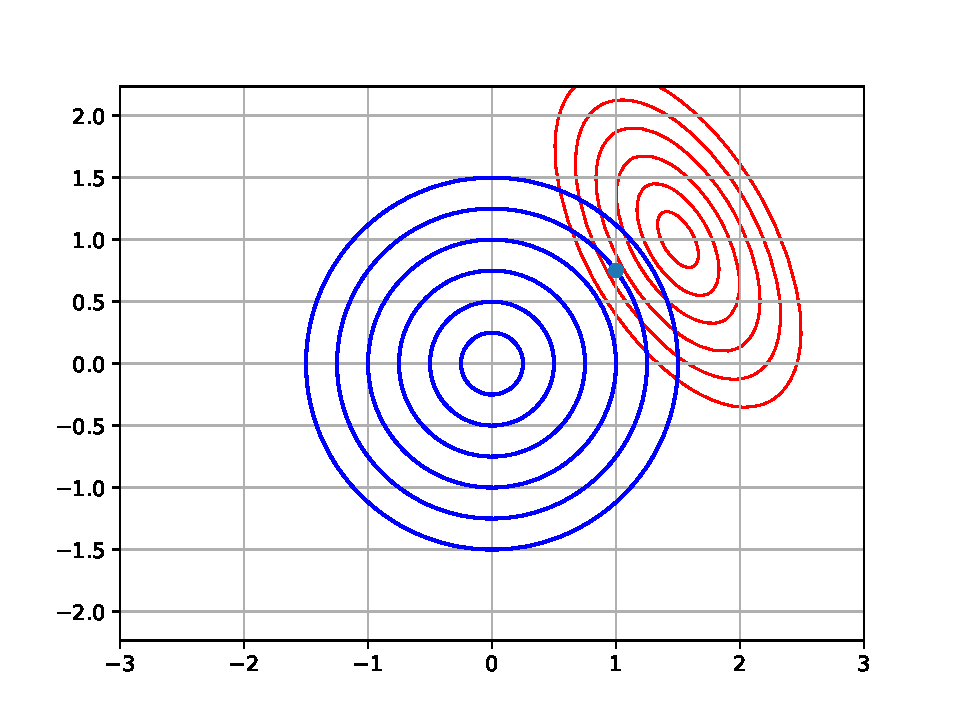
\includegraphics[width=\textwidth]{sparse/l2_ball} \\
      \(l_2\)-penalty \\
      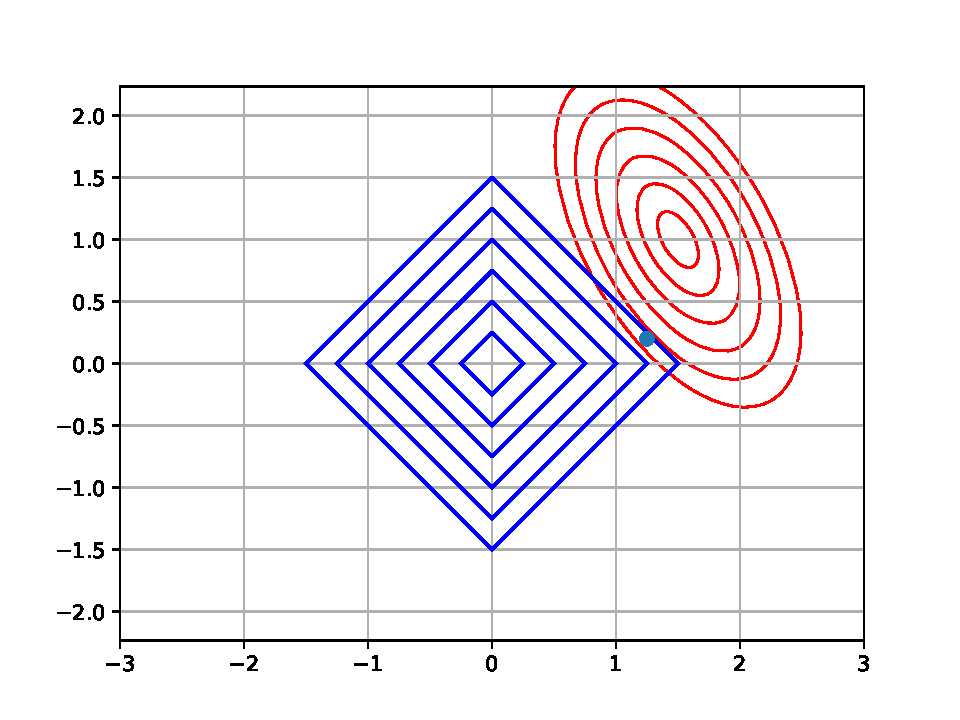
\includegraphics[width=\textwidth]{sparse/l1_ball} \\
      \(l_1\)-penalty
    \end{column}

    \begin{column}{0.25\textwidth}
      \centering
      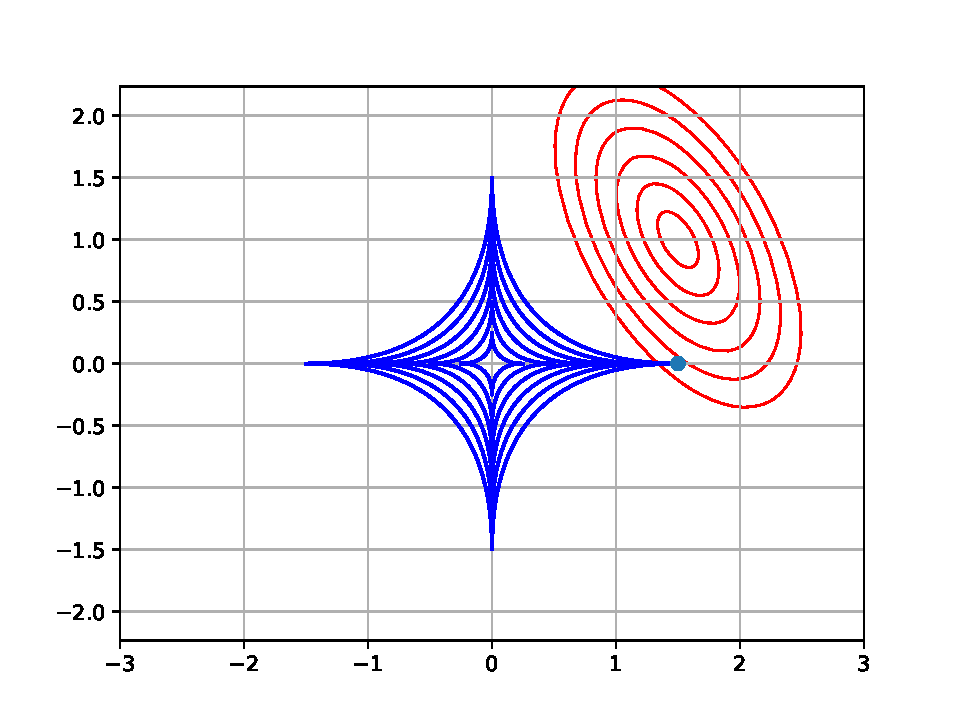
\includegraphics[width=\textwidth]{sparse/l12_ball} \\
      \(l_{1/2}\)-penalty \\
      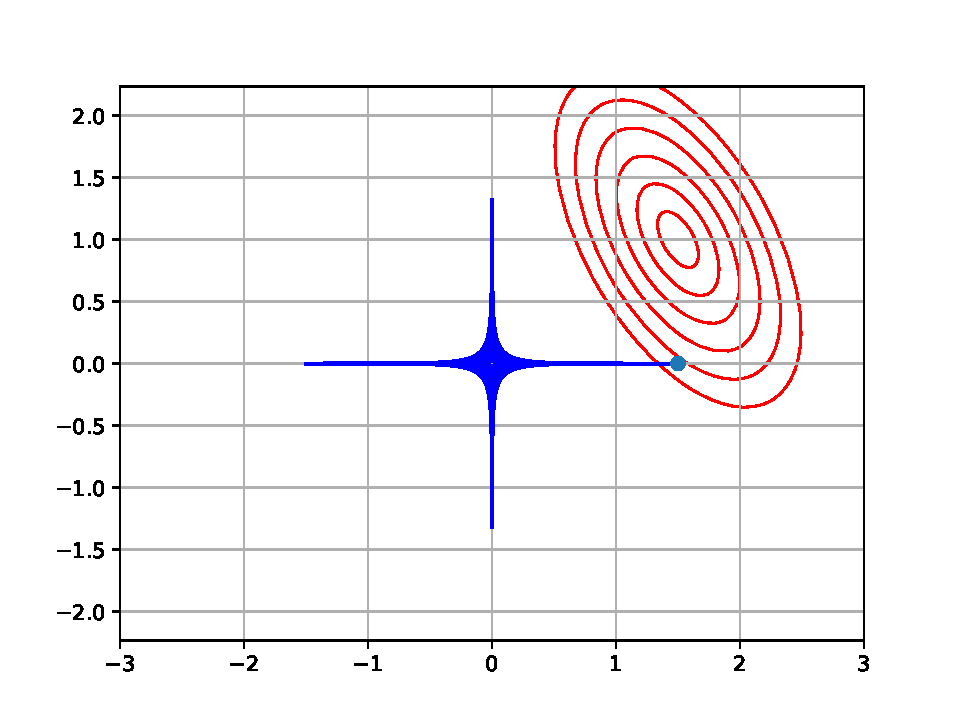
\includegraphics[width=\textwidth]{sparse/l18_ball} \\
      \(l_{1/8}\)-penalty
    \end{column}
  \end{columns}
\end{frame}

\begin{frame}{Sparse Bayesian regression}
  Add \alert{sparsity-inducing prior}
  \begin{columns}
    \begin{column}{0.5\textwidth}
      \centering
      \begin{block}{Strong sparsity}
        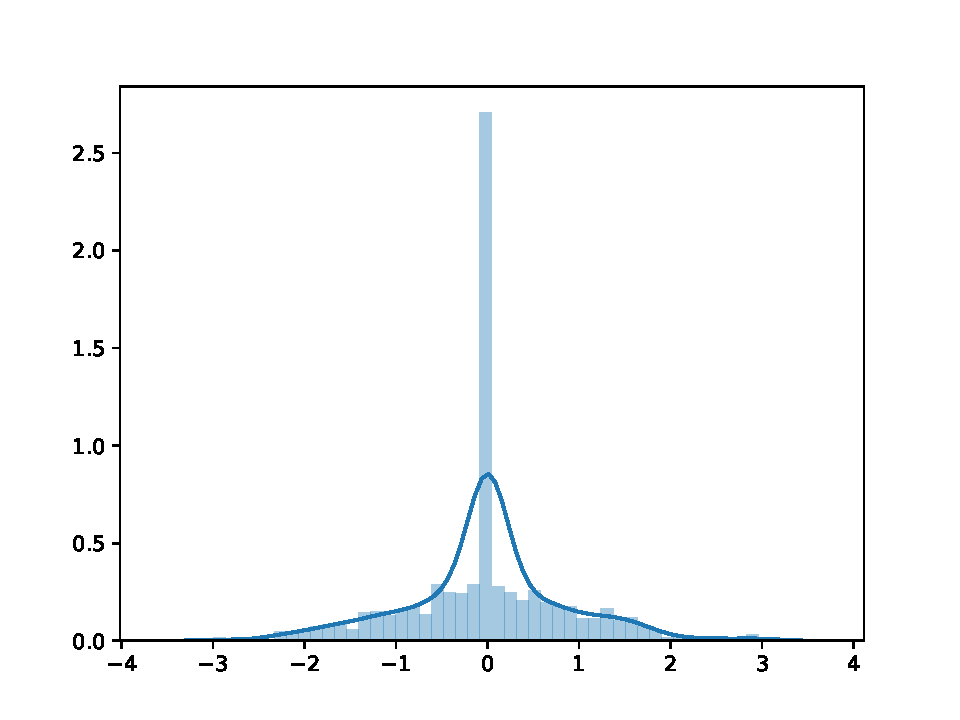
\includegraphics[width=0.75\textwidth]{sparse/strong_sparse}
        \begin{align*}
          \beta_d &\sim (1 - z_d) \mathcal{N}(0, \sigma^2) + z_d \delta_0 \\
          z_d & \sim \text{Ber}(\omega)
        \end{align*}
        \begin{itemize}
          \item probability of exact zero
          \item discrete variables
        \end{itemize}
      \end{block}
    \end{column}

    \begin{column}{0.5\textwidth}
      \centering
      \begin{block}{Weak sparsity}
        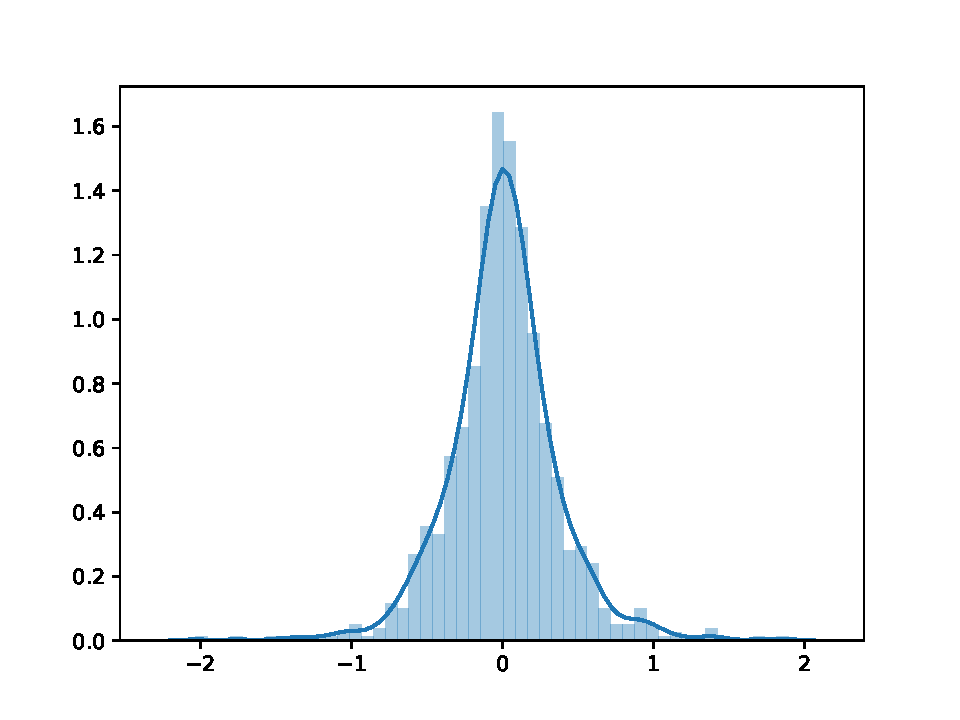
\includegraphics[width=0.75\textwidth]{sparse/weak_sparse}
        \begin{align*}
          \beta_d & \sim \mathcal{N}(0, \sigma^2_d) \\
          \sigma^2_d & \sim \text{IG}(a)
        \end{align*}
        \begin{itemize}
          \item continuous at zero
          \item continuous variables
        \end{itemize}
      \end{block}
      \end{column}
    \end{columns}
\end{frame}

\begin{frame}{Problem}
      \centering
      Build a model that estimates \(\boldsymbol\beta \) from observations \(\mathbf{y}\) such that \(\mathbf{y} = \mathbf{X} \boldsymbol\beta + \boldsymbol\varepsilon\), and elements of \(\boldsymbol\beta \) contain zeros. 
\end{frame}

%\begin{frame}{Problem}
%      \centering
%      Train a model {\color{red}\cancel{on $N$ data examples $\mathbf{B}, \mathbf{Y}$}} that estimates \(\boldsymbol\beta \) from observations \(\mathbf{y}\) such that \(\mathbf{y} = \mathbf{X} \boldsymbol\beta + \boldsymbol\varepsilon\), and elements of \(\boldsymbol\beta \) contain zeros. 
%\end{frame}

%\begin{frame}{LISTA}
%  \begin{itemize}
%    \item Represent iterative soft-thresholding algorithm as a recurrent neural network with shared weights
%    \item Learn weights with backpropagation through time
%    \item {\color{red}Overfitting}
%    \item {\color{red}No uncertainty estimation}
%  \end{itemize}
%\end{frame}

\begin{frame}{Iterative Shrinkage-Thresholding Algorithm (ISTA)}
\begin{block}{Soft thresholding}
\begin{equation*}
  h_\lambda(\mathbf{b}) = \text{sgn}(\mathbf{b}) \max(|\mathbf{b}| - \lambda, 0),
  \end{equation*}
\end{block}
 \begin{columns}
    \begin{column}{0.4\textwidth}
          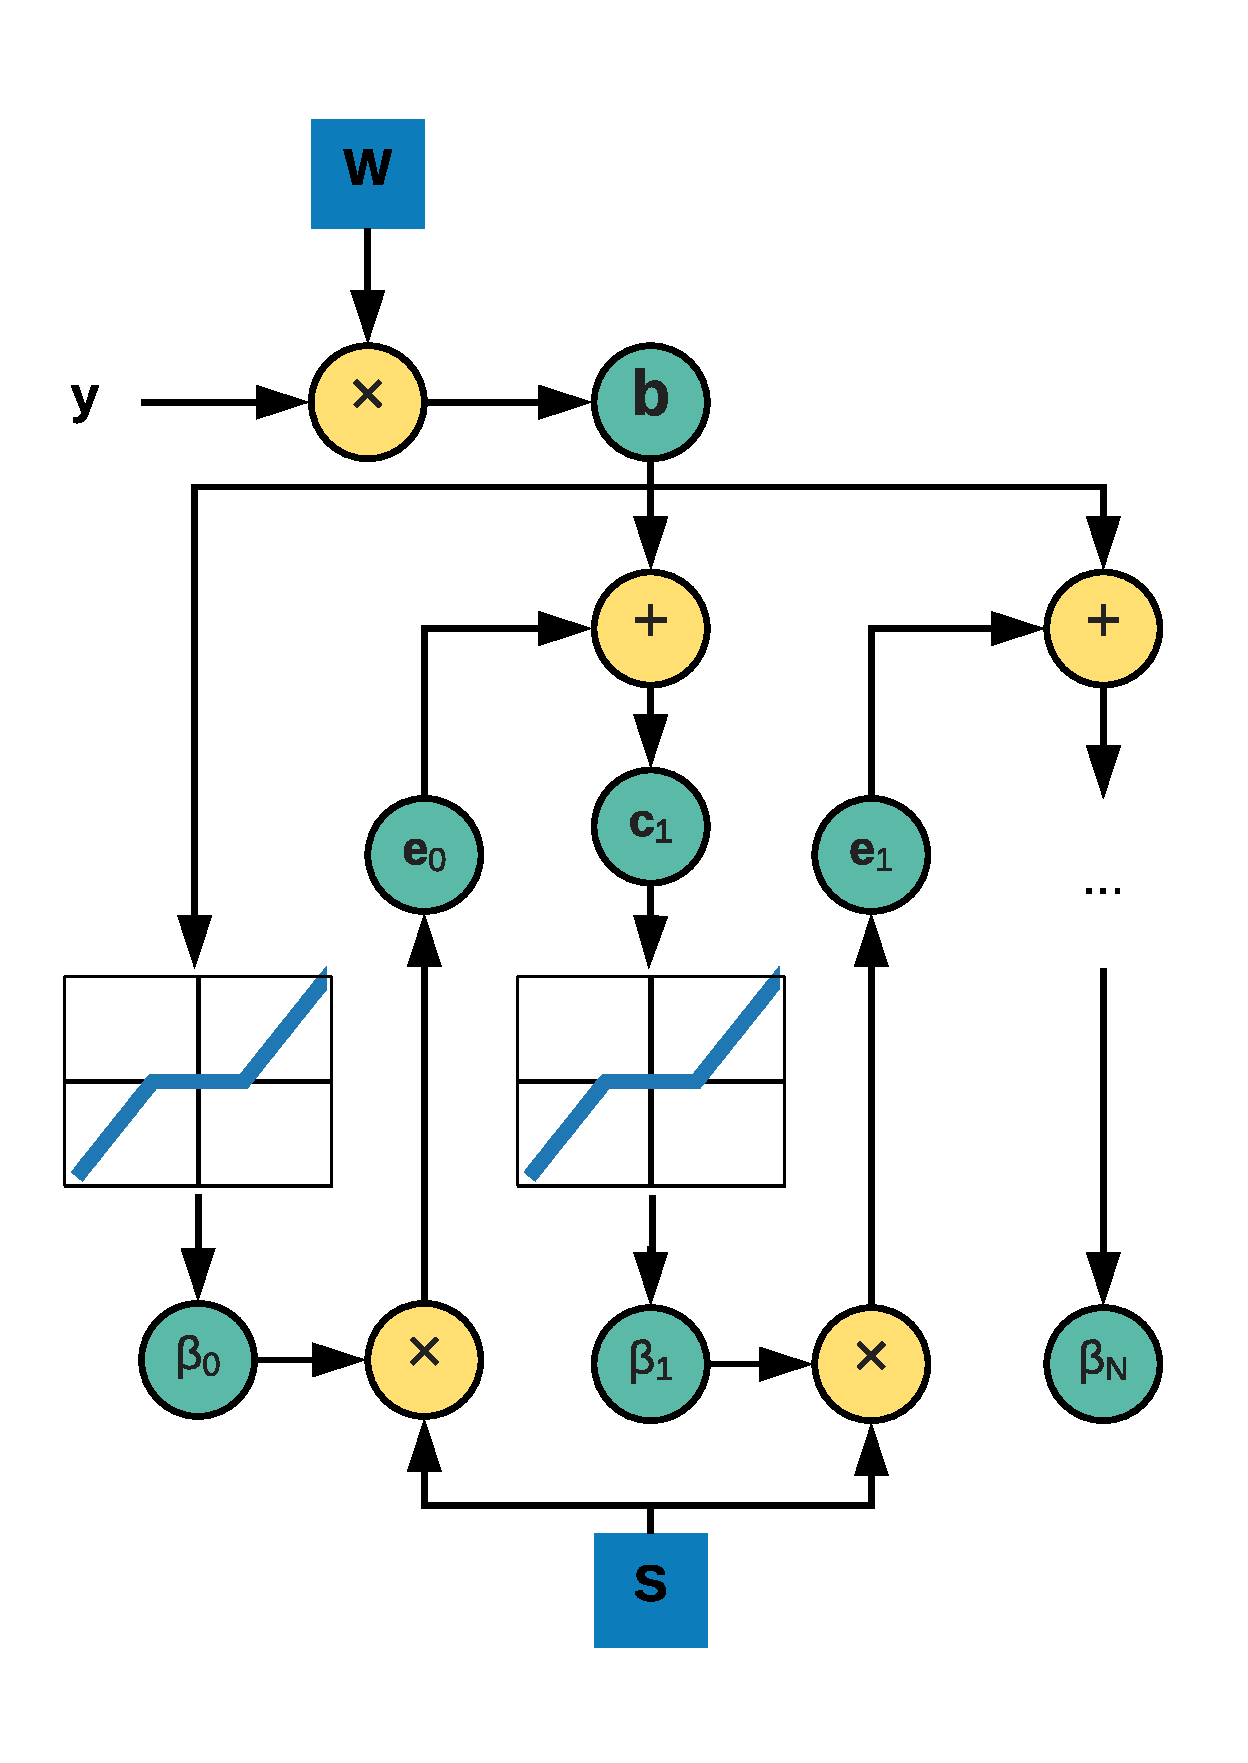
\includegraphics[width=0.75\columnwidth]{graphics/LISTA_main.pdf}
    \end{column}
    \begin{column}{0.6\textwidth}
    \begin{block}{Prediction}
    \begin{algorithmic}[1]
      \REQUIRE observation $\mathbf{y}$
      \STATE \textit{Define.} weights $\mathbf{W} = \mathbf{X}^\top/E$, $E$ --- the largest eigenvalue of $\mathbf{X}^\top\mathbf{X}$ and $\mathbf{S} = \mathbf{I}_{D\times D} - \mathbf{W}\mathbf{X}$.
      \STATE \textit{Initialisation.} Dense layer $\mathbf{b} \gets \mathbf{W}\mathbf{y}$
      \STATE \textit{Initialisation.} Soft-thresholding nonlinearity $\widehat{\boldsymbol\beta}_0 \gets h_\lambda(\mathbf{b})$
      \REPEAT
      \STATE Dense layer $\mathbf{c}_l \gets \mathbf{b} + \mathbf{S}\widehat{\boldsymbol\beta}_{l-1}$
      \STATE Soft-thresholding nonlinearity $\widehat{\boldsymbol\beta}_{l} \gets h_\lambda(\mathbf{c}_l)$
      \UNTIL{converged}
      \RETURN $\widehat{\boldsymbol\beta} \gets \widehat{\boldsymbol\beta}_{L}$
    \end{algorithmic}
    \end{block}
        \end{column}
      \end{columns}
      \footnotesize{Daubechies I., Defrise M., De Mol C. An iterative thresholding algorithm for linear inverse problems with a sparsity constraint. Communications on pure and applied mathematics, 2004.}
\end{frame}
%
%\begin{frame}{Iterative Shrinkage-Thresholding Algorithm (ISTA)}
%\begin{block}{soft thresholding}
%\begin{equation*}
%  h_\lambda(\mathbf{b}) = \text{sgn}(\mathbf{b}) \max(|\mathbf{b}| - \lambda, 0),
%  \end{equation*}
%\end{block}
% \begin{columns}
%    \begin{column}{0.4\textwidth}
%          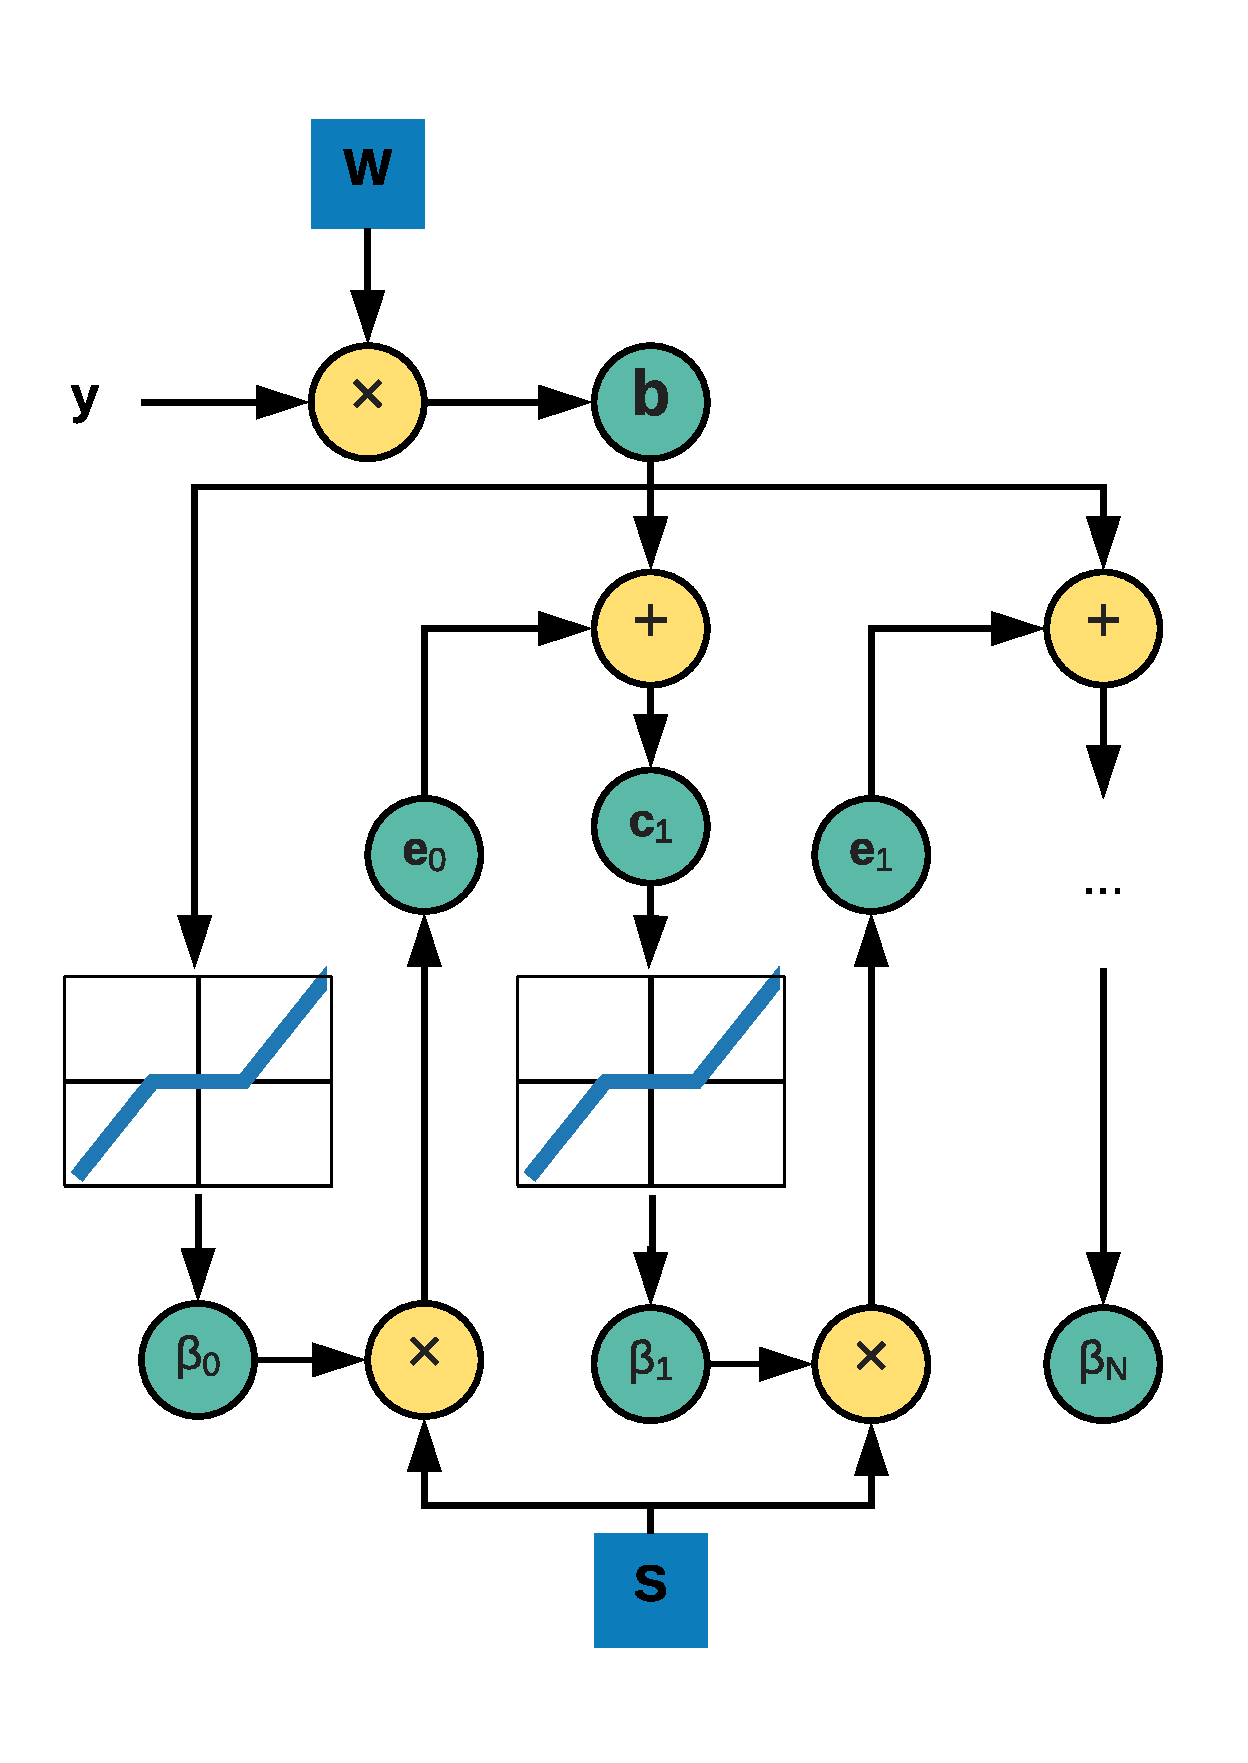
\includegraphics[width=0.75\columnwidth]{graphics/LISTA_main.pdf}
%    \end{column}
%    \begin{column}{0.6\textwidth}
%    \begin{block}{prediction}
%    \begin{algorithmic}[1]
%      \REQUIRE observation $\mathbf{y}$, number of iterations $L$
%      \STATE \textit{Define.} weights {\color{red}$\mathbf{W} = \mathbf{X}^\top/E$}, $E$ --- the largest eigenvalue of $\mathbf{X}^\top\mathbf{X}$ and {\color{red}$\mathbf{S} = \mathbf{I}_{D\times D} - \mathbf{W}\mathbf{X}$}.
%      \STATE \textit{Initialisation.} Dense layer $\mathbf{b} \gets \mathbf{W}\mathbf{y}$
%      \STATE \textit{Initialisation.} Soft-thresholding nonlinearity $\widehat{\boldsymbol\beta}_0 \gets h_\lambda(\mathbf{b})$
%      \FOR{$l=1$ \TO $L$}
%      \STATE Dense layer $\mathbf{c}_l \gets \mathbf{b} + \mathbf{S}\widehat{\boldsymbol\beta}_{l-1}$
%      \STATE Soft-thresholding nonlinearity $\widehat{\boldsymbol\beta}_{l} \gets h_\lambda(\mathbf{c}_l)$
%      \ENDFOR
%      \RETURN $\widehat{\boldsymbol\beta} \gets \widehat{\boldsymbol\beta}_{L}$
%    \end{algorithmic}
%    \end{block}
%        \end{column}
%      \end{columns}
%      \footnotesize{Daubechies I., Defrise M., De Mol C. An iterative thresholding algorithm for linear inverse problems with a sparsity constraint. Communications on pure and applied mathematics, 2004.}
%\end{frame}

\begin{frame}{Problem}
      \centering
      {\color{red}Train a model on $N$ data examples $\mathbf{B}, \mathbf{Y}$} that estimates \(\boldsymbol\beta \) from observations \(\mathbf{y}\) such that \(\mathbf{y} = \mathbf{X} \boldsymbol\beta + \boldsymbol\varepsilon\), and elements of \(\boldsymbol\beta \) contain zeros. 
\end{frame}

\begin{frame}{Learned ISTA (LISTA)}
\begin{block}{}
Learn weights $\mathbf{W}, \mathbf{S}$ based on training data
\end{block}
 \begin{columns}
    \begin{column}{0.4\textwidth}
          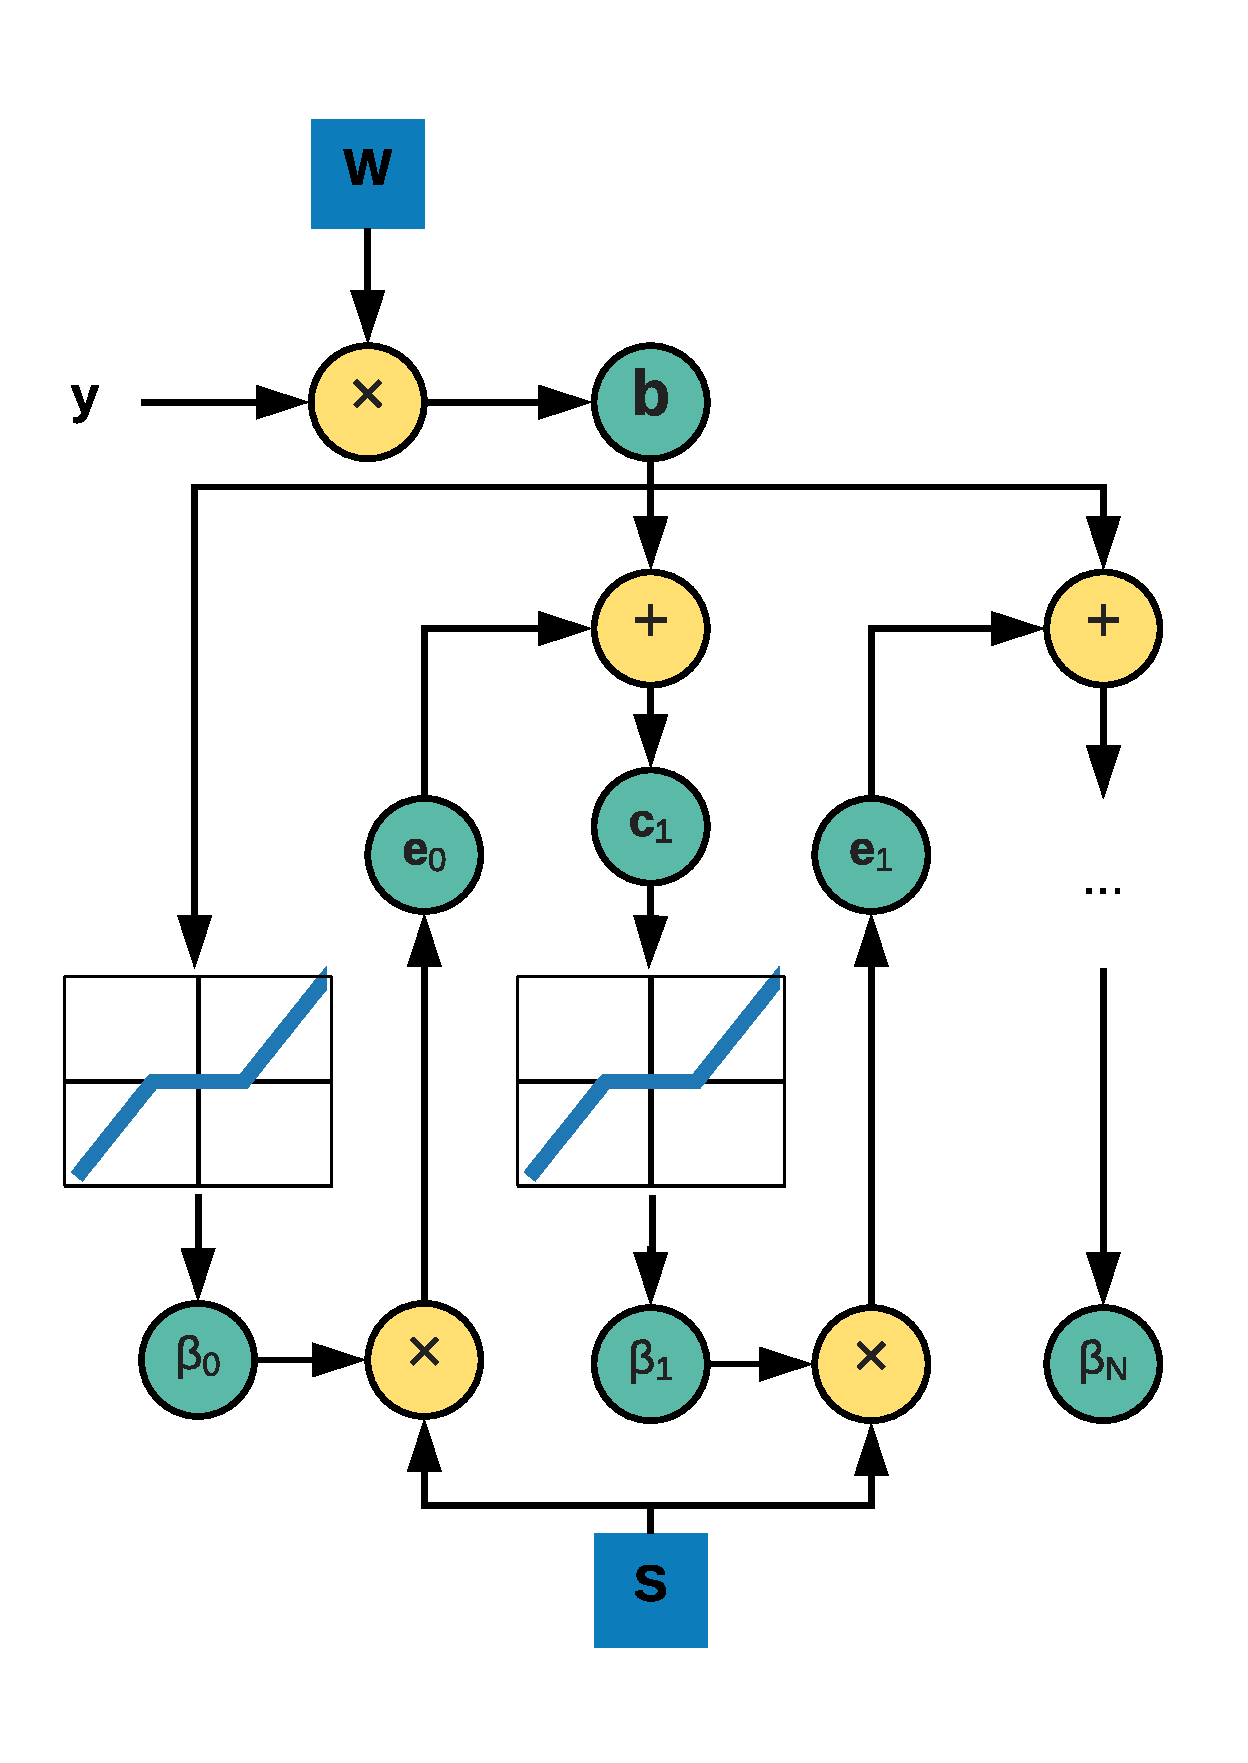
\includegraphics[width=0.75\columnwidth]{graphics/LISTA_main.pdf}
    \end{column}
    \begin{column}{0.6\textwidth}
    \begin{block}{Forward pass}
    \begin{algorithmic}[1]
      \REQUIRE observation $\mathbf{y}$, {\color{red}current weights $\mathbf{W}, \mathbf{S}$, current $\lambda$, number of layers $L$}
      \STATE \textit{Initialisation.} Dense layer $\mathbf{b} \gets \mathbf{W}\mathbf{y}$
      \STATE \textit{Initialisation.} Soft-thresholding nonlinearity $\widehat{\boldsymbol\beta}_0 \gets h_\lambda(\mathbf{b})$
      \FOR{{\color{red}$l=1$ \TO $L$}}
      \STATE Dense layer $\mathbf{c}_l \gets \mathbf{b} + \mathbf{S}\widehat{\boldsymbol\beta}_{l-1}$
      \STATE Soft-thresholding nonlinearity $\widehat{\boldsymbol\beta}_{l} \gets h_\lambda(\mathbf{c}_l)$
      \ENDFOR
      \RETURN $\widehat{\boldsymbol\beta} \gets \widehat{\boldsymbol\beta}_{L}$
    \end{algorithmic}
    \end{block}
    \begin{block}{Backward pass}
     \begin{algorithmic}[1]
      \STATE {\color{red}update $\mathbf{W}, \mathbf{S}, \lambda$ based on derivatives of the mean squared loss}
       \end{algorithmic}
    \end{block}
        \end{column}
      \end{columns}
      \footnotesize{Gregor, K., LeCun, Y. Learning fast approximations of sparse coding. ICML 2010}
\end{frame}

\section[Proposed model]{Proposed model}
\subsection[Model]{Model}
\begin{frame}{BayesLISTA}
  \begin{block}{Prior}
    \begin{equation*}
      p(\mathbf{W}) = \prod_{d=1}^D\prod_{k=1}^K \mathcal{N}(w_{ij} ; 0, \eta^{-1}), \quad
      p(\mathbf{S}) = \prod_{d'=1}^D\prod_{d''=1}^D \mathcal{N}(s_{d'd''} ; 0, \eta^{-1}),
    \end{equation*}
    \end{block}
    \begin{block}{Forward pass}
    Propagate the distribution for $\widehat{\boldsymbol\beta}$ through layers, add Gaussian noise
    \begin{equation*}
      p(\mathbf{\boldsymbol\beta}| \mathbf{y}, \mathbf{W}, \mathbf{S}, \gamma, \lambda)
      = \prod_{d=1}^D\mathcal{N}\left(\beta_d; [\widehat{\boldsymbol\beta}(\mathbf{y} ; \mathbf{S}, \mathbf{W}, \lambda)]_d, \gamma^{-1}\right)
    \end{equation*}
    \end{block}
    \begin{block}{Posterior}
  \begin{equation*}
  p(\mathbf{W}, \mathbf{S}, \gamma, \eta | \mathbf{B}, \mathbf{Y}, \lambda)
  = \frac{p(\mathbf{B} | \mathbf{Y}, \mathbf{W},  \mathbf{S}, \gamma, \lambda) p(\mathbf{W} | \eta )p(\mathbf{S} | \eta) p(\eta) p(\gamma)}{p(\mathbf{B} | \mathbf{Y}, \lambda)}
  \end{equation*}
  \end{block}
   \begin{block}{Backward pass}
   Update weights with probabilistic backpropagation
    \end{block}
 
  \end{frame}

\subsection[Prediction]{Prediction}
  \begin{frame}{Uncertainty propagation: Initialisation}
     \begin{block}{Goal}
    \begin{itemize}
      \item[] Model intermediate latent variables with parametrised distributions
      \item[] Apply approximate Bayesian inference methods
    \end{itemize}
  \end{block}
%      The output of soft-thresholding can be approximated with the spike and slab distribution
    
      \begin{columns}
        \begin{column}{0.33\textwidth}
      1. \(\mathbf{b} = \mathbf{W}\mathbf{y}\) is Gaussian-distributed
    \end{column}
    \begin{column}{0.67\textwidth}
        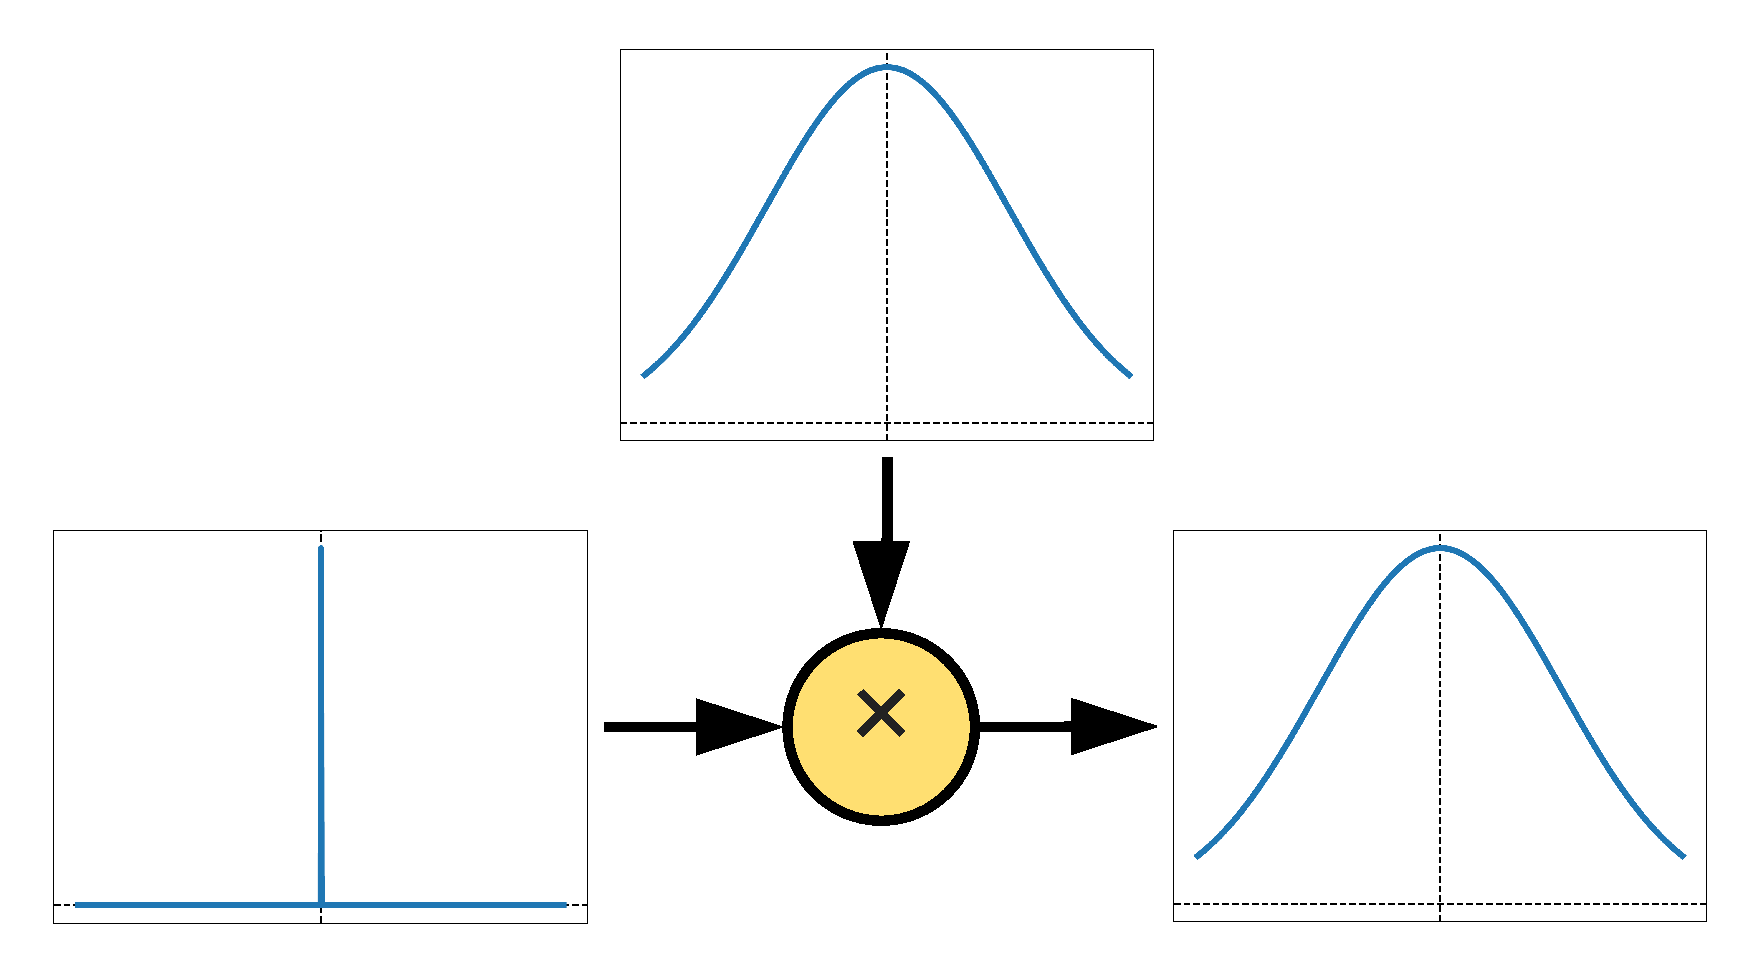
\includegraphics[width=0.6\columnwidth]{graphics/gauss_delta.pdf}
      \end{column}
    \end{columns}
    \begin{columns}
      \begin{column}{0.33\textwidth}
      2. \(\widehat{\boldsymbol\beta}_{0} = h_\lambda(\mathbf{b})\) is approximated with the spike and slab distribution
    \end{column}
    \begin{column}{0.67\textwidth}
        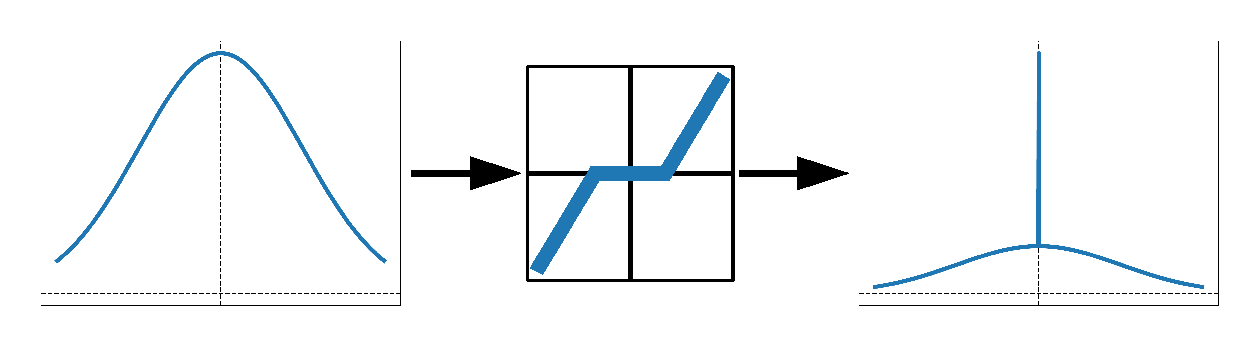
\includegraphics[width=0.6\columnwidth]{graphics/spsl_propagation.pdf}
      \end{column}
    \end{columns}
\end{frame}

\begin{frame}{Uncertainty propagation: Iterations}
    \begin{columns}
      \begin{column}{0.33\textwidth}
      3. \(\mathbf{e}_l = \mathbf{S}\widehat{\boldsymbol\beta}_{l-1}\) is approximated with the Gaussian distribution
    \end{column}
    \begin{column}{0.67\textwidth}
        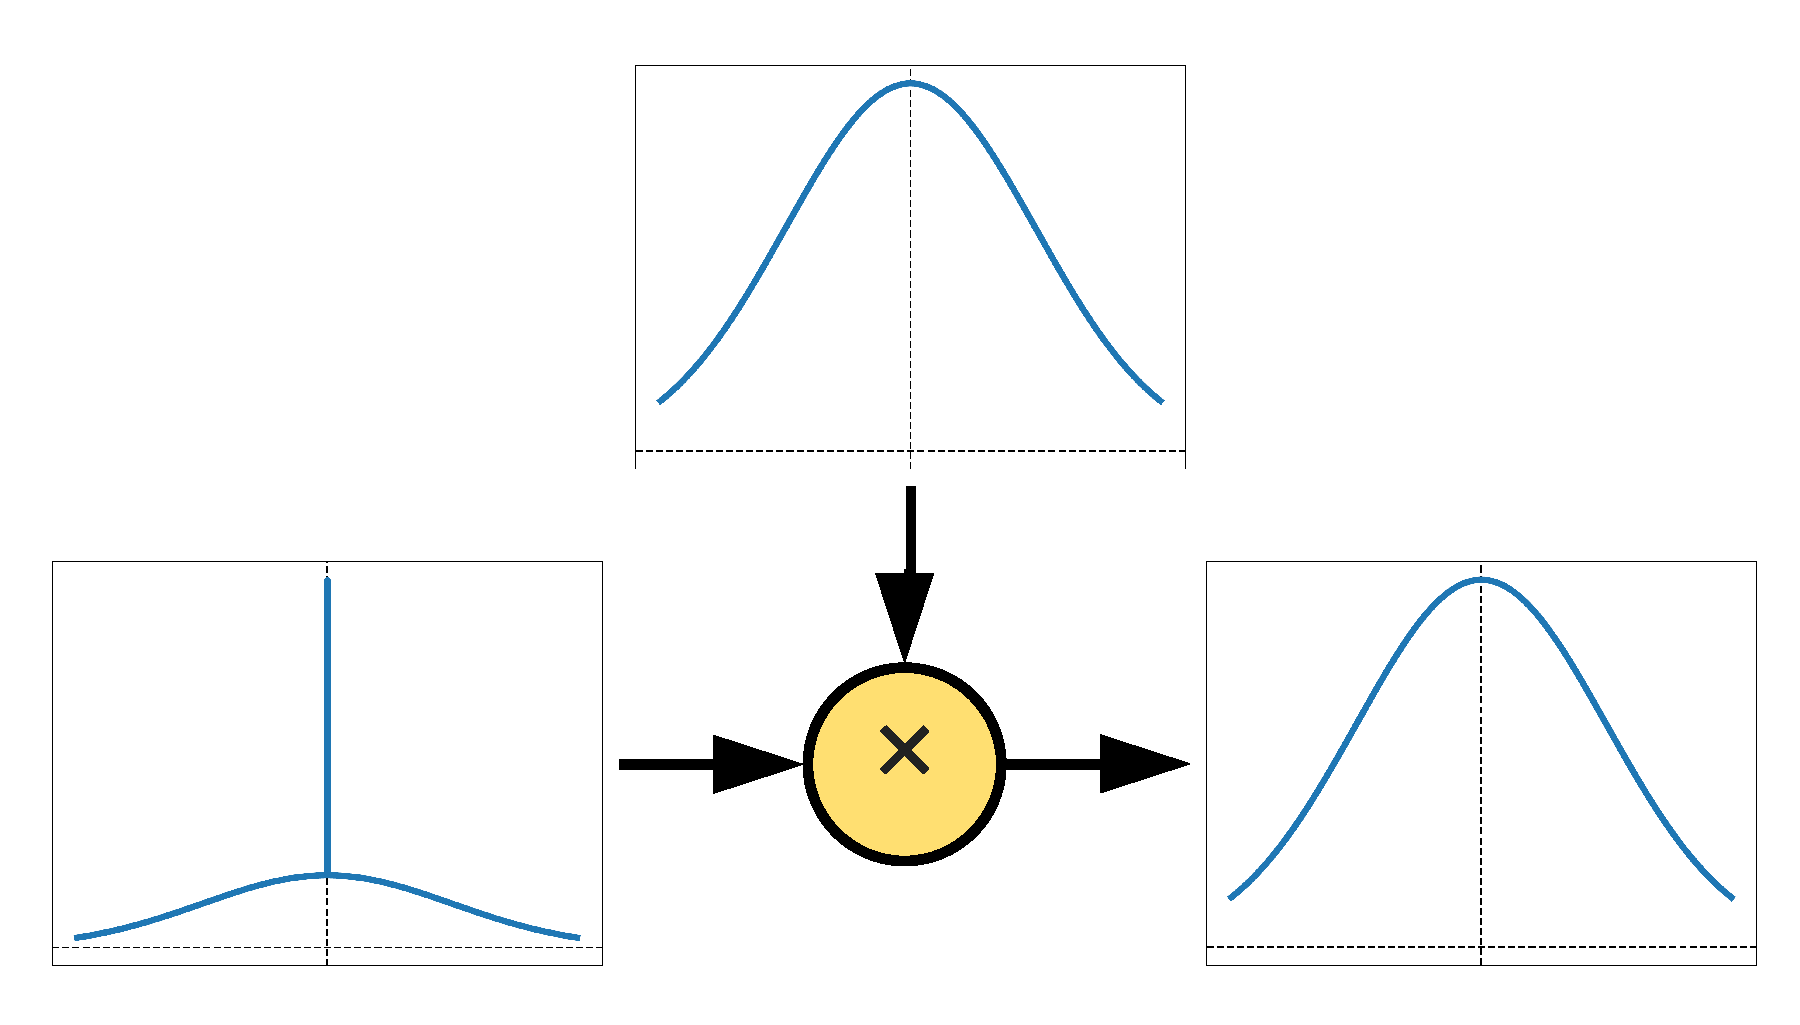
\includegraphics[width=0.6\columnwidth]{graphics/gauss_spsl.pdf}
      \end{column}
    \end{columns}
    \begin{columns}
      \begin{column}{0.33\textwidth}
      4. \(\mathbf{c}_l = \mathbf{b} + \mathbf{e}_l\) is Gaussian-distributed
    \end{column}
    \begin{column}{0.67\textwidth}
        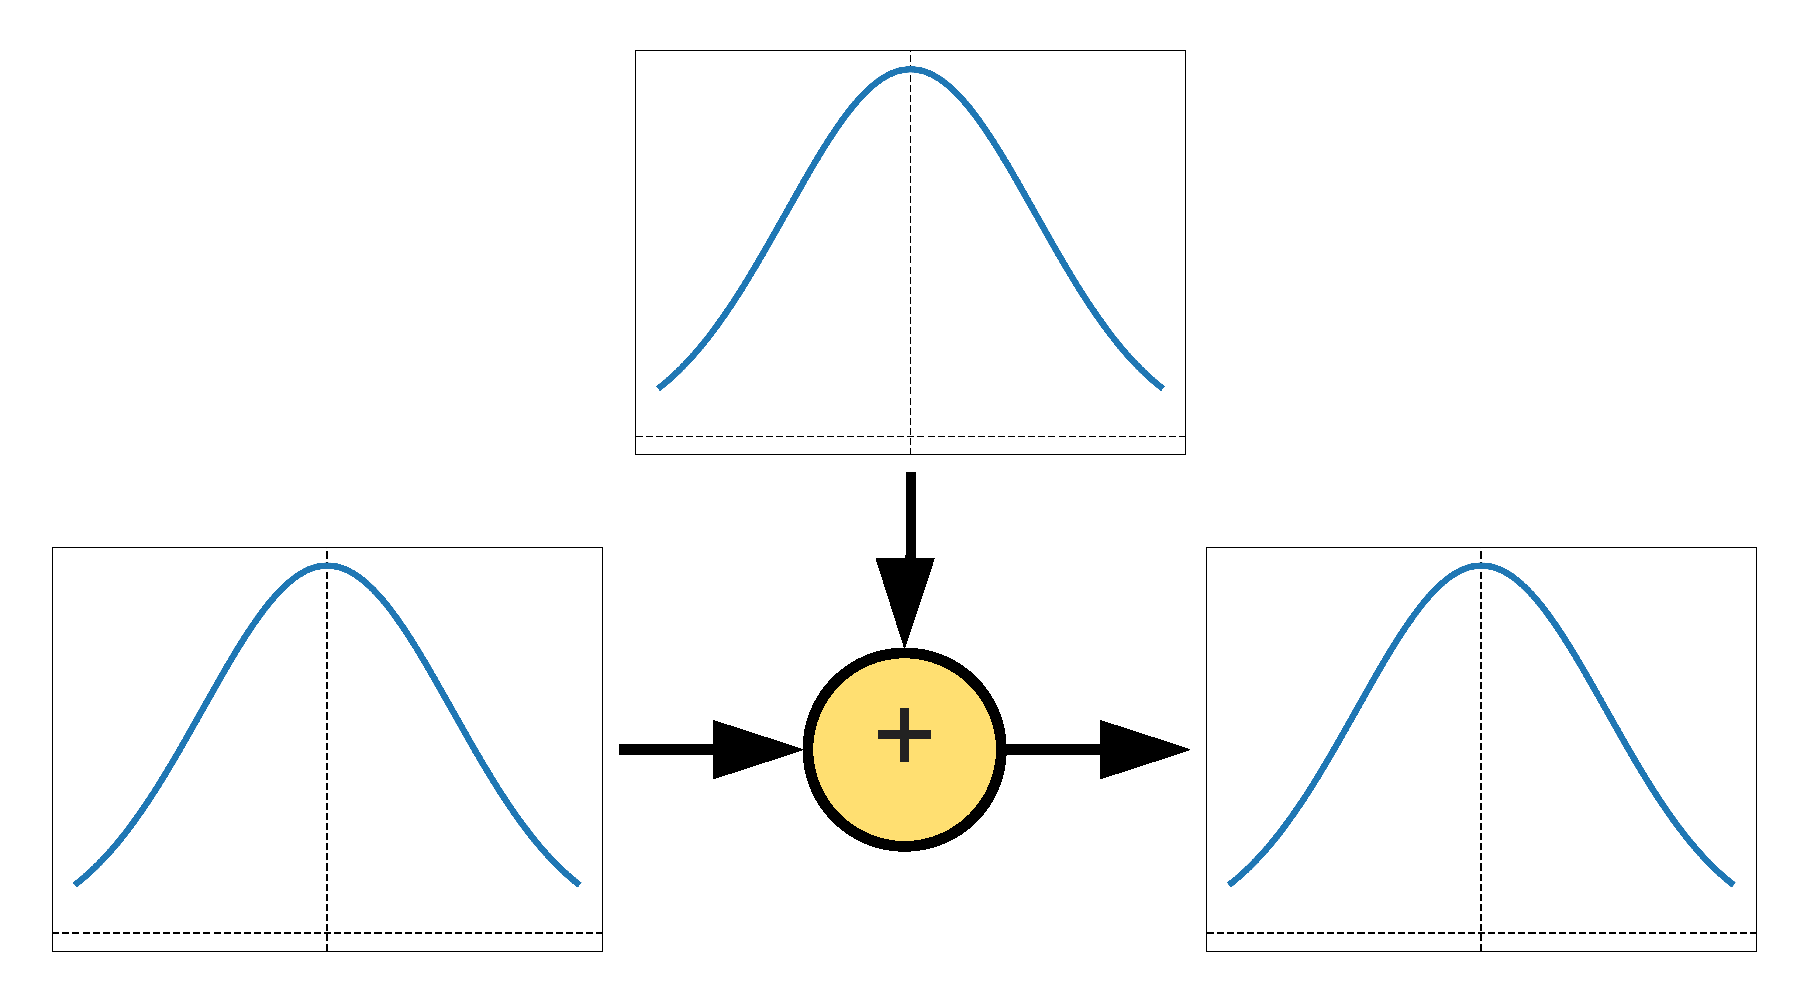
\includegraphics[width=0.6\columnwidth]{graphics/gauss_gauss.pdf}
      \end{column}
    \end{columns}
    \begin{columns}
      \begin{column}{0.33\textwidth}
      5. \(\widehat{\boldsymbol\beta}_{l} = h_\lambda(\mathbf{c}_l)\) is approximated with the spike and slab distribution
    \end{column}
    \begin{column}{0.67\textwidth}
        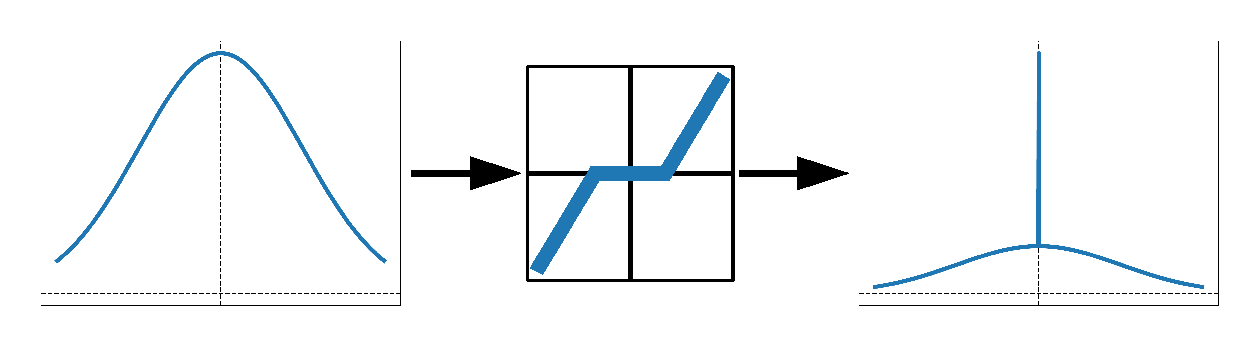
\includegraphics[width=0.6\columnwidth]{graphics/spsl_propagation.pdf}
      \end{column}
    \end{columns}
\end{frame}

\begin{frame}{Approximation quality}
    \begin{columns}
      \begin{column}{0.5\textwidth}
       \centering
       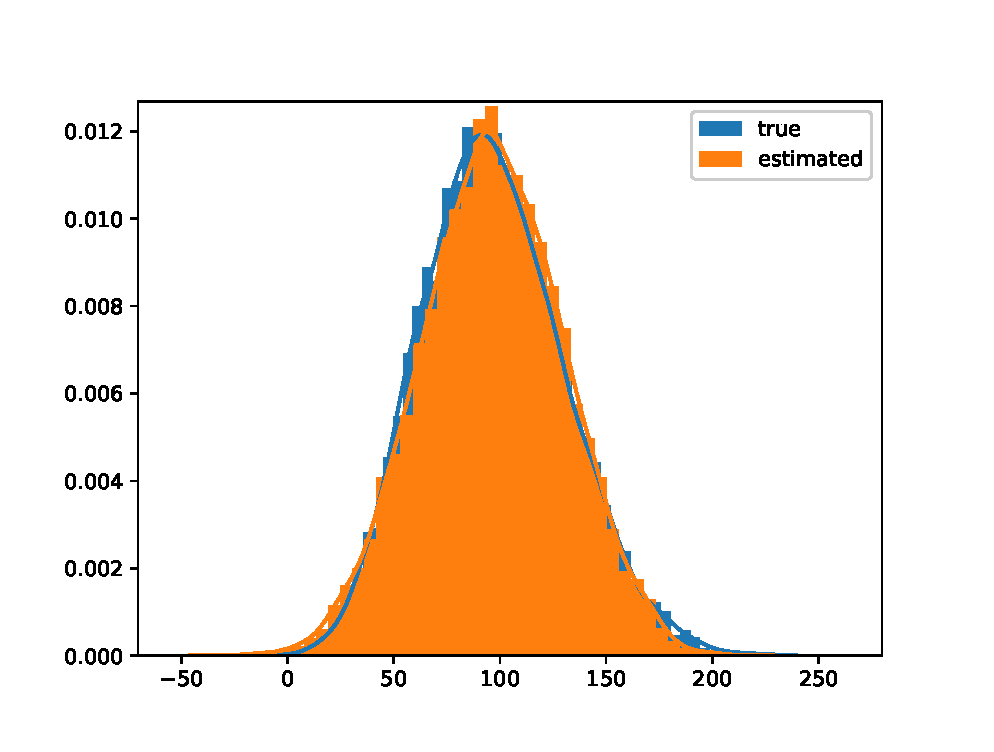
\includegraphics[width=\columnwidth]{graphics/d_testing}\\
       Approximation of the \newline product of Gaussian and spike and slab distributions
      \end{column}
            \begin{column}{0.5\textwidth}
      \centering
      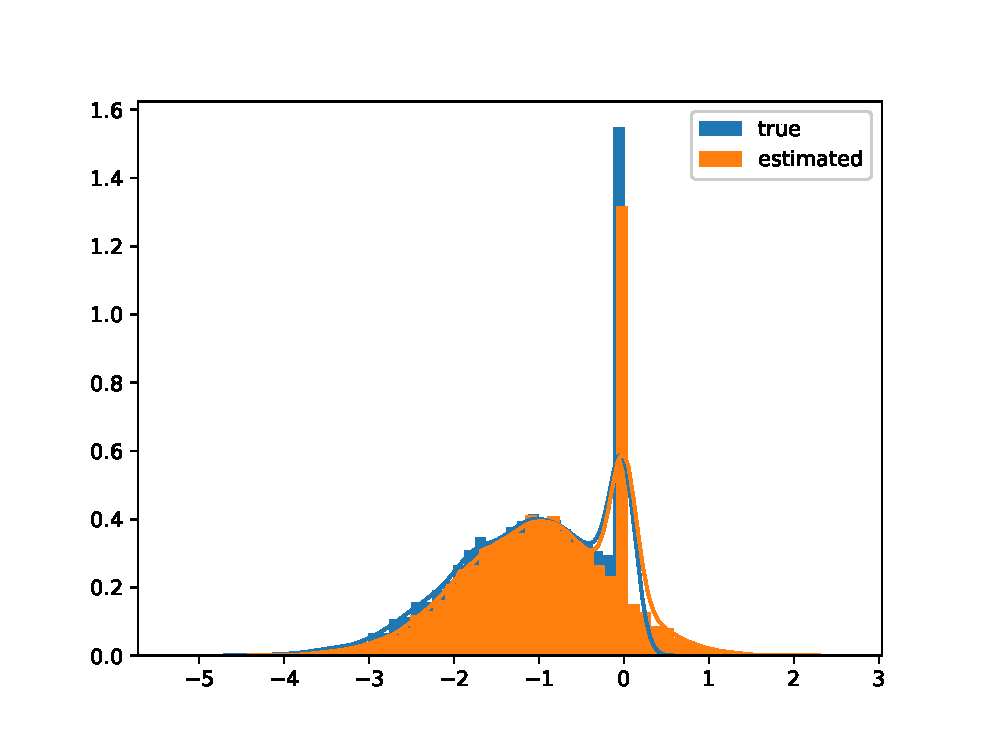
\includegraphics[width=\columnwidth]{graphics/z_new_testing}\\
      Approximation of the propagation through soft thresholding
      \end{column}
      \end{columns}

\end{frame}

\subsection[Inference]{Inference}
\begin{frame}{Probabilistic backpropagation}
\begin{block}{Posterior}
 \begin{equation*}
  p(\mathbf{W}, \mathbf{S}, \gamma, \eta | \mathbf{B}, \mathbf{Y}, \lambda)
  = \frac{p(\mathbf{B} | \mathbf{Y}, \mathbf{W},  \mathbf{S}, \gamma, \lambda) p(\mathbf{W} | \eta )p(\mathbf{S} | \eta) p(\eta) p(\gamma)}{p(\mathbf{B} | \mathbf{Y}, \lambda)}
  \end{equation*}
  \end{block}

\begin{block}{Approximate posterior}
\begin{align*}
\begin{split}
q(\mathbf{W}, \mathbf{S}, \gamma, \eta) &= \prod_{d=1}^D\prod_{k=1}^K \mathcal{N}(w_{dk} ; m^w_{dk}, v^w_{dk}) \prod_{d'=1}^D\prod_{d''=1}^D \mathcal{N}(s_{d'd''} ; m^s_{d'd''}, v^s_{d'd''}) \\
&\times \text{Gam}(\gamma; a^\gamma, b^\gamma) \text{Gam}(\eta; a^\eta, b^\eta)
\end{split}
\end{align*}
  \end{block}

\begin{block}{Assumed density filtering (ADF)}
Iteratively add factors from the posterior $p$ one-by-one in the factorised approximating distribution $q$ and update the approximation $q$. 
\end{block}

\footnotesize{Hernandez-Lobato, J. M., Adams, R. Probabilistic backpropagation for scalable learning of Bayesian neural networks, ICML 2015}
\end{frame}

\begin{frame}{Probabilistic backpropagation}
\begin{block}{Updates for Gaussian parameters}
  \begin{equation*}
  q(a) = Z^{-1}f(a)\mathcal{N}(a; m, v) 
  \end{equation*}

For each factor $a \in \{w_{dk}, s_{d'd''}\}$ new parameters are:
  \begin{equation*}
  m\leftarrow m + v \frac{\partial \log Z}{\partial m}, \,
  v\leftarrow v - v^2\left[ \left(\frac{\partial \log Z}{\partial m}\right)^2 - 2 \frac{\partial \log Z}{\partial v}\right]
  \end{equation*}
  \alert{$\frac{\partial \log Z}{\partial m}$, $\frac{\partial \log Z}{\partial v}$ are required}
\end{block}

\begin{block}{Updates for Gamma parameters}
For each factor $a \in \{\eta, \gamma\}$ new parameters are:
  \begin{equation*}
  \alpha\leftarrow [Z_0Z_2Z_1^{-2}(\alpha+1)/\alpha -1]^{-1}, \,
  \beta\leftarrow [Z_2Z_1^{-1}(\alpha+1)/\beta - Z_1Z_0^{-1}\alpha/\beta]^{-1}
  \end{equation*}
  \alert{$Z_0 = Z(\alpha, \beta)$, $Z_1=Z(\alpha+1, \beta)$, $Z_2 = Z(\alpha+2, \beta)$ are required}
  \end{block}
\end{frame}

\begin{frame}{Probabilistic backpropagation}

The normalising constant when incorporating the likelihood factor:
    \begin{equation*}
  Z  = \int \prod_{d=1}^{D} \mathcal{N}(\beta_d ; [\widehat{\boldsymbol\beta}(\mathbf{y} ; \mathbf{S}, \mathbf{W}, \lambda)]_d, \gamma^{-1}) q(\mathbf{W}, \mathbf{S}, \gamma, \eta) \mathrm{d}\mathbf{W} \mathrm{d}\mathbf{S} \mathrm{d}\gamma \mathrm{d}\eta
  \end{equation*}
  
  Assuming the spike and slab distribution for $\widehat{\boldsymbol\beta}$:
\begin{equation*}
\label{eq:Z}
Z \approx \prod_{d=1}^D \left[\omega^{\widehat{\boldsymbol\beta}}_d  \mathcal{T}\left(\beta_d ; 0, \beta^\gamma / \alpha^\gamma, 2\alpha^\gamma\right) + \vphantom{m^{\widehat{\boldsymbol\beta}}_d} \left(1 - \omega^{\widehat{\boldsymbol\beta}}_d\right)\mathcal{N}\left(\beta_d ; m^{\widehat{\boldsymbol\beta}}_d,  \beta^\gamma / (\alpha^\gamma - 1) + v^{\widehat{\boldsymbol\beta}}_d\right)\right],
\end{equation*}
  where $\{\omega^{\widehat{\boldsymbol\beta}}_d, m^{\widehat{\boldsymbol\beta}}_d, v^{\widehat{\boldsymbol\beta}}_d\}$ are the parameters of the spike and slab distribution for $[\widehat{\boldsymbol\beta}]_d$.
  


\end{frame}

\section{Experiments}
\begin{frame}{Synthetic Experiments}
  \centering
  \begin{block}{}
    \begin{columns}
      \begin{column}{0.5\textwidth}
        \centering
        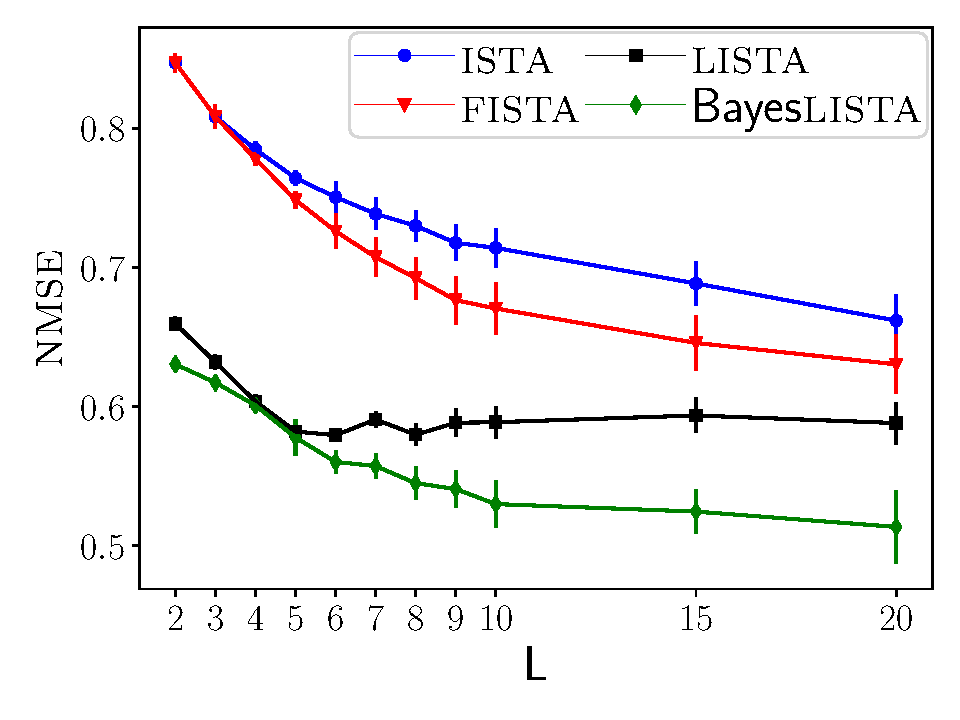
\includegraphics[width=0.75\columnwidth]{graphics/synthetic_number_of_layers/nmse_validation} \\
        Different depth performance
      \end{column}
      \begin{column}{0.5\textwidth}
        \centering
        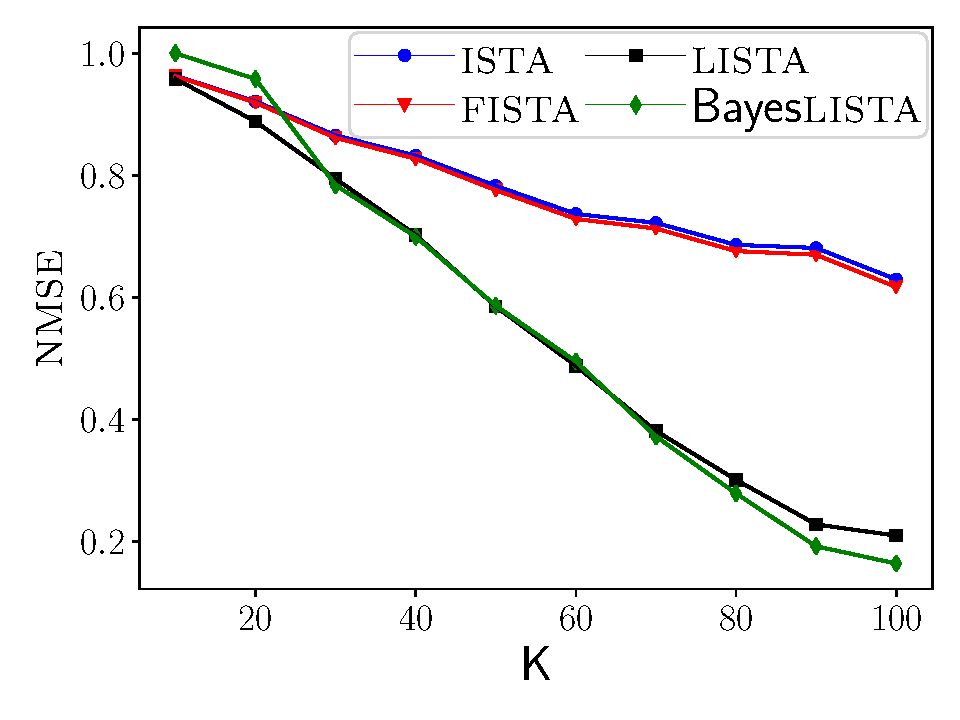
\includegraphics[width=0.75\columnwidth]{graphics/synthetic_undersampling/nmse_validation} \\
        Different observation size performance
      \end{column}
    \end{columns}
  \end{block}
  $N_\text{train} = 1000$, $D = 100$, $p(\beta_d==0) = 0.8$, $\eta^{-1} = 0.25$, $\lambda=0.1$
\end{frame}

\begin{frame}{MNIST Experiments}
  \centering
%    \begin{block}{Results for increasing number of iterations for observation size K=100 and K=250}
%    \begin{columns}
%    \begin{column}{0.33\textwidth}
%    \centering
%    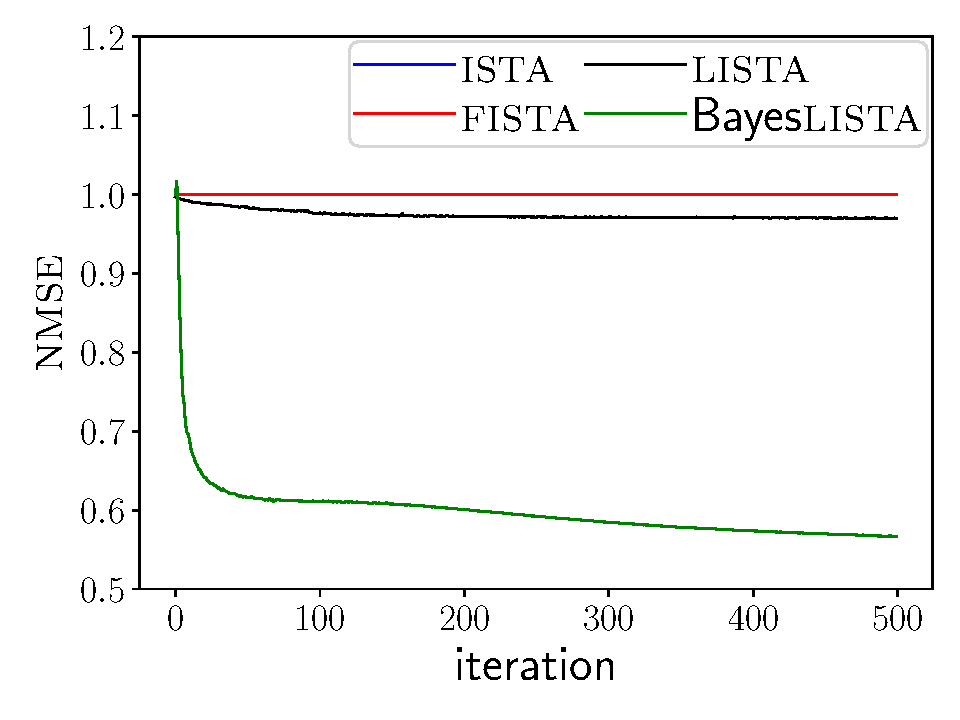
\includegraphics[width=0.75\columnwidth]{graphics/mnist/100_nmse_valid.pdf} \\
%    NMSE, $K=100$
%    \end{column}
%    \begin{column}{0.33\textwidth}
%    \centering
%    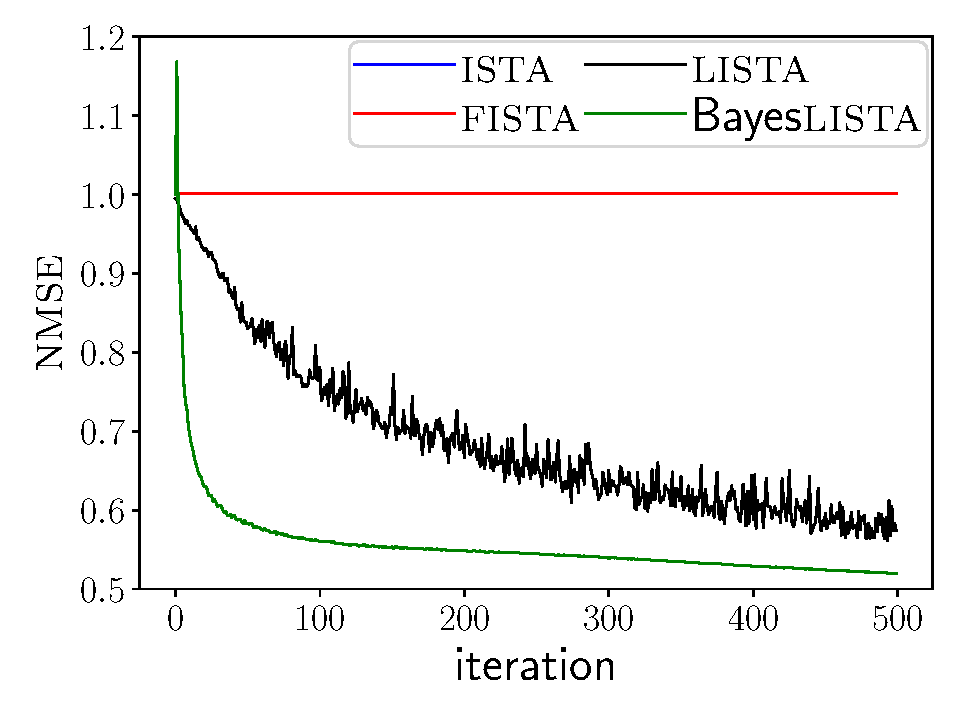
\includegraphics[width=0.75\columnwidth]{graphics/mnist/250_nmse_valid.pdf} \\
%    NMSE, $K=250$
%    \end{column}
%    \end{columns}
%    \end{block}
$\mathbf{X}$ - random i.i.d, $D = 784$, $K=100$
  \begin{block}{Posterior parameters for an image of digit 7}
    \begin{columns}
      \begin{column}{0.33\textwidth}
        \centering
        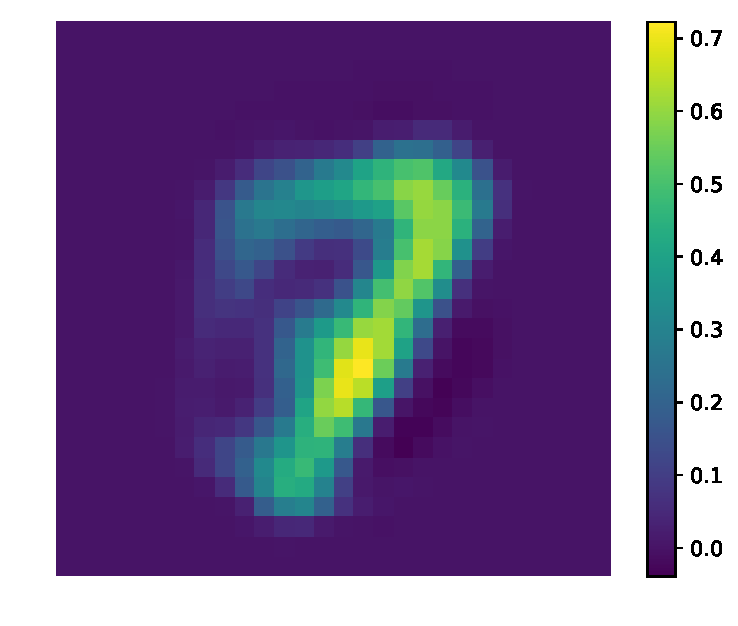
\includegraphics[width=0.75\columnwidth]{graphics/posterior_mean} \\
        \(\boldsymbol\beta \) posterior mean
      \end{column}
      \begin{column}{0.33\textwidth}
        \centering
        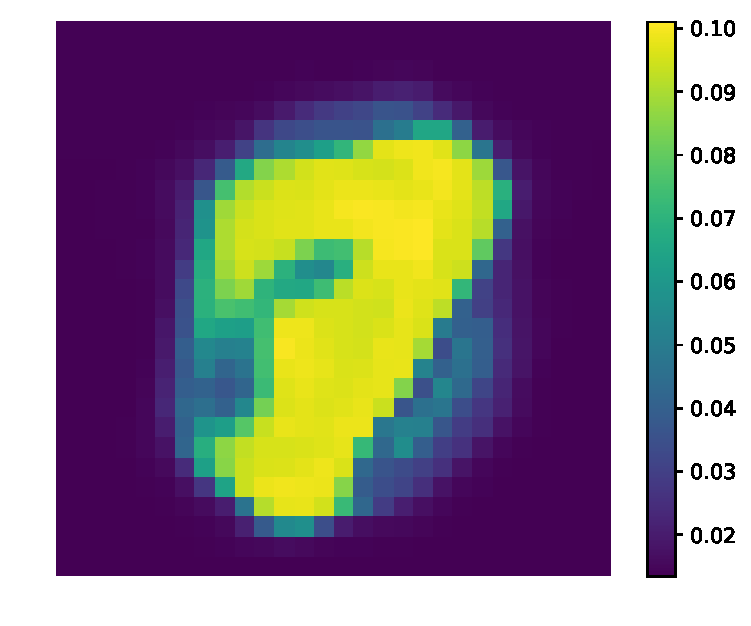
\includegraphics[width=0.75\columnwidth]{graphics/posterior_std}\\
        \(\boldsymbol\beta \) posterior std
      \end{column}
      \begin{column}{0.33\textwidth}
        \centering
        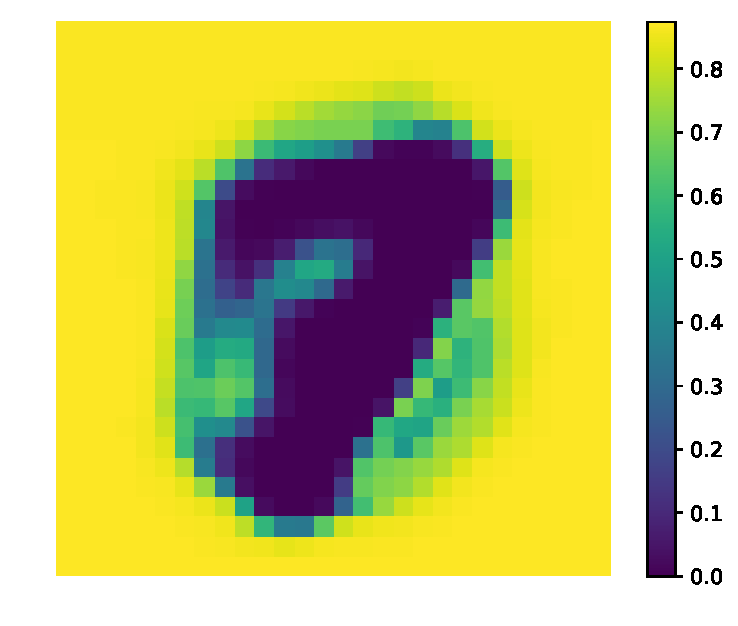
\includegraphics[width=0.75\columnwidth]{graphics/posterior_spike_indicator}\\
        \(\boldsymbol\beta \) posterior spike indicator
      \end{column}
    \end{columns}
  \end{block}

  \centering
  \begin{block}{Samples from the posterior for an image of digit 7}
    \begin{columns}
      \begin{column}{0.33\textwidth}
        \centering
        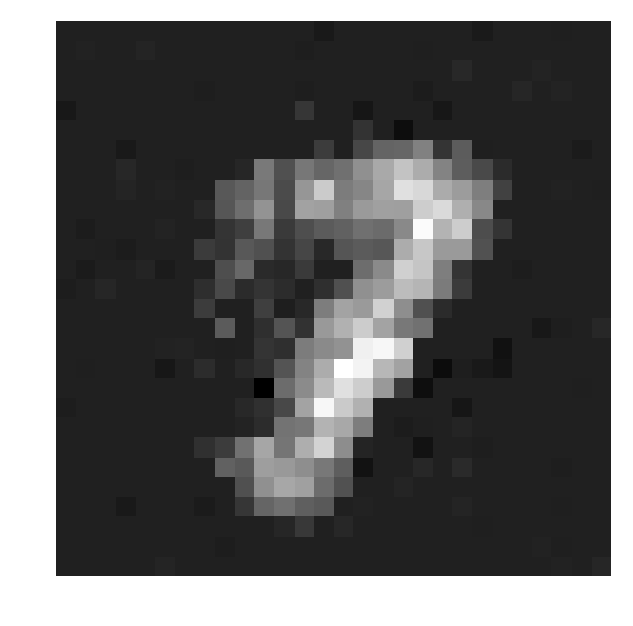
\includegraphics[width=0.75\columnwidth]{graphics/posterior_sample_0}
      \end{column}
      \begin{column}{0.33\textwidth}
        \centering
        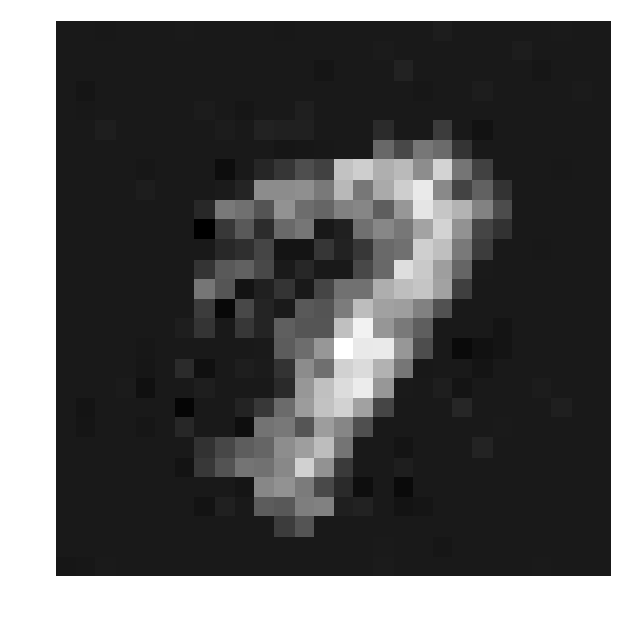
\includegraphics[width=0.75\columnwidth]{graphics/posterior_sample_1}
      \end{column}
      \begin{column}{0.33\textwidth}
        \centering
        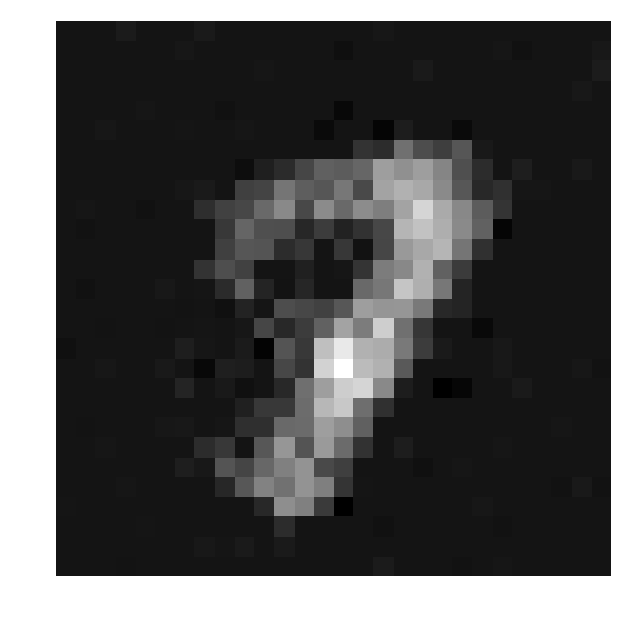
\includegraphics[width=0.75\columnwidth]{graphics/posterior_sample_2}
      \end{column}
    \end{columns}
  \end{block}
\end{frame}

\begin{frame}{Active Learning}
  \centering
  \begin{block}{Idea}
    Use the estimated uncertainty to choose next training data with largest variance
  \end{block}
  $N_\text{train} = 50$, $N_\text{pool} = 500$, $N_\text{addition}=1$
  \begin{columns}
    \begin{column}{0.5\textwidth}
      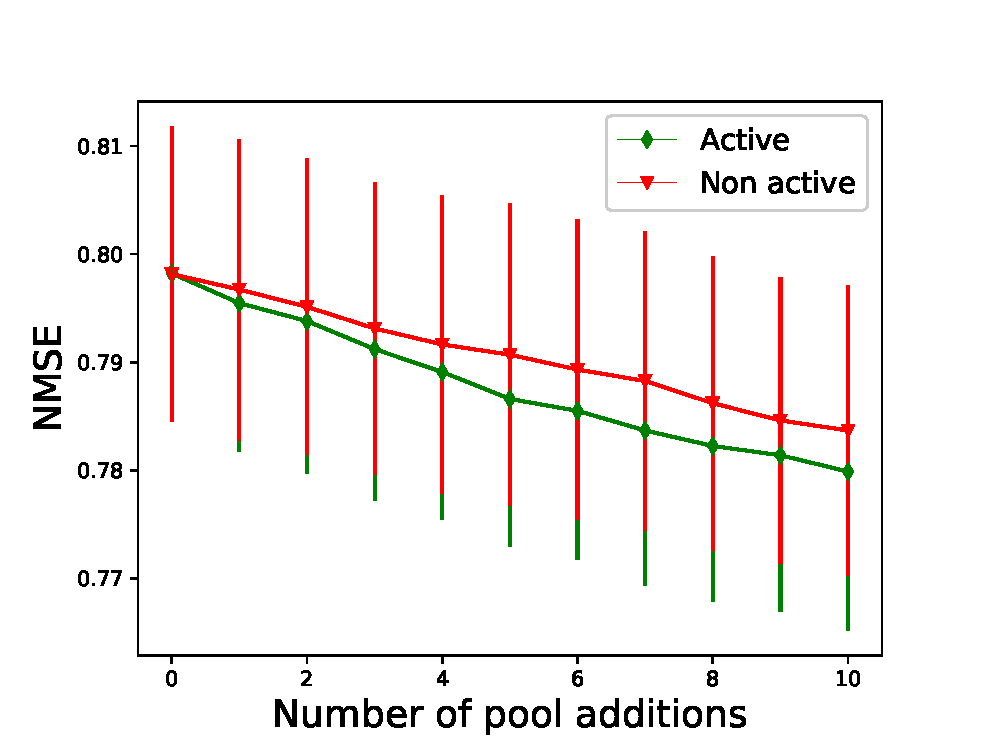
\includegraphics[width=1.0\columnwidth]{graphics/active_mnist/nmse_validation}
    \end{column}
    % \begin{column}{0.5\textwidth}
    %   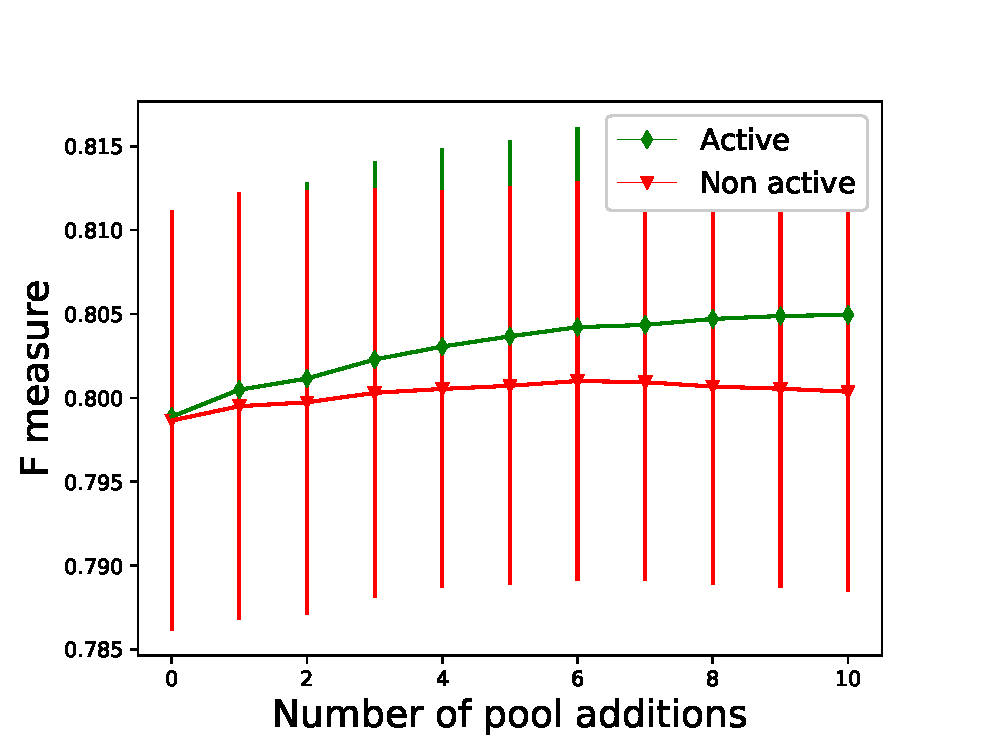
\includegraphics[width=1.0\columnwidth]{graphics/active_mnist/f_measure_validation}
    % \end{column}
  \end{columns}

\end{frame}

\section{Conclusions}
\begin{frame}{Contributions and future work}
\begin{block}{Key contributions}
  \begin{itemize}
   \item Bayesian version of LISTA
    \item Uncertainty propagation to make inference feasible
    \item Uncertainty quantification, for example, for active learning
  \end{itemize}
\end{block}
  \begin{block}{Future work}
    \begin{itemize}
      \item The shrinkage parameter $\lambda$ as a parameter of the model
      \item Stochastic inference
    \end{itemize}
  \end{block}
  \begin{block}{}
  Code will be available at danilkuzin.github.io
  \end{block}
\end{frame}


\end{document}
